\documentclass[parskip=full,11pt,twoside]{scrartcl}

\usepackage[l2tabu,orthodox]{nag}
\usepackage[utf8]{inputenc}

\titlehead{\centering
\includegraphics[width=6cm]{img/logo.pdf}}
\title{Wavelength}
\subtitle{$\bm{\lambda}$-IDE}
\author{Muhammet Guemues, Markus Himmel, Marc Huisinga,\\Philip Klemens, Julia Schmid, Jean-Pierre von der Heydt}

% section numbers in margins:
\renewcommand\sectionlinesformat[4]{\makebox[0pt][r]{#3}#4}

% header & footer
\usepackage{scrlayer-scrpage}
\lofoot{\today}
\refoot{\today}
\pagestyle{scrheadings}

\usepackage[sfdefault,light]{roboto}
\usepackage[T1]{fontenc}
\usepackage[ngerman]{babel}
\usepackage{datetime2}
\usepackage[hidelinks]{hyperref}
\usepackage[nameinlink]{cleveref}
\crefname{figure}{Abb.}{Abb.}
\usepackage[section]{placeins}
\usepackage{xcolor}
\usepackage{graphicx}
\hypersetup{
	pdftitle={Pflichtenheft},
	bookmarks=true,
}
\usepackage{csquotes}

\usepackage{amsmath}
\usepackage{bm}
\usepackage{mathtools}
\usepackage{amssymb}
\usepackage{float}
\usepackage{subcaption}

\usepackage{glossaries}
\GlsSetQuote{+}
%
\usepackage{pkg/pflichtenheft}

\MakeOuterQuote{"}

\makeglossaries

\newglossaryentry{lk}
{ 
	name=$\lambda$-Kalkül,
	description={Der $\lambda$-Kalkül ist eine formale Sprache, die, basierend auf Funktionsdefinitionen, eine systematische Untersuchung von Funktionen zulässt}
}
\newglossaryentry{lapp}
{ 
	name=$\lambda$-Applikation,
	plural=$\lambda$-Applikationen,
	description={Applikationen stellen die Anwendung eines \gls{lt}s auf einen weiteren \gls{lt} dar. Sie haben im Allgemeinen die Form: \emph{<\gls{lt}1> <\gls{lt}2>}, wobei die spitzen Klammern hier nur der Übersicht wegen eingefügt wurden und im eigentlichen 			    Ausdruck nicht vorkommen}
}
\newglossaryentry{labs}
{ 
	name=$\lambda$-Abstraktion,
	plural=$\lambda$-Abstraktionen,
	description={Abstraktionen stellen eine Funktionsdefinition einer Funktion in einer Variablen dar. Abstraktionen haben die Form \emph{$\lambda$} <\gls{var}>.<\gls{lt}>, wobei die Ausdrücke in den spitzen Klammern inklusive der spitzen Klammern durch die entsprechenden Objekte zu ersetzen sind}
}
\newglossaryentry{lt}
{
	name=$\lambda$-Term,
	plural=$\lambda$-Terme,
	description={Terme im \gls{lk} sind entweder \emph{\glspl{lapp}} oder \emph{\glspl{labs}} oder \emph{\glspl{var}}}
}
\newglossaryentry{var}
{ 
	name=Variable,
	plural=Variablen,
	description={Variablen sind Platzhalter für konkrete Werte. Als Variablen zugelassen sind beliebige Zeichen und Zeichenkombinationen bis auf die folgenden:
	\begin{tabular} {| l | c | r |}
	\hline
	 $\lambda$ & . & \textbackslash \\
	 \hline
	\end{tabular}
	}
}
\newglossaryentry{alpha} 
{
	name=$\alpha$-Konversion,
	description={Die $\alpha$-Konversion entspricht einer Variablenumbenennung in einer \gls{lapp}. \underline{Beispiel:} Umbenennung von x in y: $\lambda x.T \stackrel{\alpha}{\Rightarrow} \lambda y.T[y/x]$}
}
\newglossaryentry{beta}
{
	name=$\beta$-Reduktion,
	plural=$\beta$-Reduktionen,
	description={Die $\beta$-Reduktion entspricht einer Funktionsauswertung. Sie ist nur auf \glspl{redex} anwendbar.
			Sollten durch die Auswertung freie Variablen gebunden werden, so müssen diese vorher durch \gls{alpha} in ungenutzte Variablen umbenannt werden.
	 		Formal gilt für eine Variable $V$ und \glspl{lt} $T_1$ und $T_2$ die \gls{subs}: $(\lambda V.T_1) T_2 \stackrel{\beta}{\Rightarrow} T_1[T_2/V]$}
}
\newglossaryentry{redex} 
{
	name=Redex,
	plural=Redexe,
	description={Redexe (Reducible Expressions) sind Ausdrücke der Form \emph{($\lambda$.\gls{lt}1) \gls{lt}2}}
}
\newglossaryentry{fv} 
{
	name=freie Variable,
	plural=freie Variablen,
	description={Eine Variable in einem \gls{lt} heißt \emph{frei}, wenn sie kein Parameter einer \gls{labs} ist}
}
\newglossaryentry{gv} 
{
	name=gebundene Variable,
	plural=gebundene Variablen,
	description={Eine Variable in einem \gls{lt} heißt \emph{gebunden}, wenn sie Parameter einer \gls{labs} ist}
}
\newglossaryentry{subs}
{
	name=Substitution,
	plural=Substitutionen,
	description={Bei einer Substitution einer \glspl{var} $y$ in einer \gls{labs} $\lambda x.T_1$, wobei $T_1$ ein \gls{lt} ist,  werden alle freien Vorkommen von $x$ in $T_1$ durch $y$ ersetzt und der Parameter in y umbenannt. 
			In Formeln: $\lambda x.T_1 \stackrel{\text{Substitution mit $y$}}{\Longrightarrow}\lambda y.[T_1/y]$}
}
\newglossaryentry{aws}
{
	name=Auswertungsstrategie,
	plural=Auswertungsstrategien,
	description={Eine Auswertungsstrategie ist ein Algorithmus, der bestimmt, wie ein \gls{lt} ausgewertet wird. Dabei kann es vorkommen, dass eine Auswertungsstrategie bei der Auswertung eines \gls{lt} in eine Endlosschleife gerät, während eine andere 				Strategie terminiert}
}
\newglossaryentry{nr}
{
	name=normale Reduktionsordnung,
	description={Die normale Reduktionsordnung ist eine \gls{aws}, bei der immer der linkeste äußerste \gls{redex} zuerst $\beta$-reduziert wird}
}
\newglossaryentry{cbn}
{
	name=Call by Name,
	description={Call by Name ist eine \gls{aws}, bei der der linkeste äußerste \gls{redex}, der nicht von einem $\lambda$ umgeben ist, zuerst $\beta$-reduziert wird}
}
\newglossaryentry{cbv}
{
	name=Call by Value,
	description={Call by Value ist eine \gls{aws}, bei der der linkeste äußerste \gls{redex}, der nicht von einem $\lambda$ umgeben ist und dessen Argument ein konkreter Wert ist, zuerst $\beta$-reduziert wird.}
}
\newglossaryentry{yc} 
{
	name=Y-Kombinator,
	description={Formal dient der Y-Kombinator dazu, \gls{rec} zu ermöglichen. Er ist definiert als: $Y \coloneqq \lambda f.(\lambda x.f(x\,x))(\lambda x.f(x\,x))$}
}	
\newglossaryentry{rec}
{
	name=Rekursion,
	description={Eine Funktion heißt rekursiv, wenn sie sich selbst aufruft. Der Aufruf wird dann als Rekursion bezeichnet}
}
\newglossaryentry{brow}
{
	name=kompatibler Browser,
	plural=kompatible Browser,
	description={Als kompatible Browser gelten die folgenden:
	\begin{itemize}
	\item Microsoft Edge ab Version 41.16299.15.0
	\item Mozilla Firefox ab Version 57.0
	\item Google Chrome ab Version 62.0.3202
	\end{itemize}}
}
\newglossaryentry{ao}
{
	name=Applicative Order,
	description={Eine \gls{aws}, bei der der rechteste innerste Redex zuerst $\beta$-reduziert wird}
}
\newglossaryentry{mfe}
{
	name=Mehrfacheinrückung,
	plural=Mehrfacheinrückungen,
	description={Mehrfacheinrückungen ergänzen die \glspl{st} um verschiedene Einrückungsebenen}
}
\newglossaryentry{st}
{
	name=Smart Tab,
	plural=Smart Tabs,
	description={Bei einem Zeilenwechsel wird die neue Zeile genauso eingerückt wie die alte Zeile}
}

\newglossaryentry{vls}
{
	name={vereinfachte $\lambda$-Syntax},
	description={Variante der herkömmlichen Syntax des \glslink{lk}{$\lambda$-Kalküls},
	bei der das $\lambda$-Symbol durch ein \texttt{\textbackslash}-Symbol ersetzt wird}
}

\newglossaryentry{cn}
{
	name=Church-Zahl,
	plural=Church-Zahlen,
	description={Gängige Umsetzung der natürlichen Zahlen inklusive der Null im \gls{lk}. $n\in\mathbb{N}_0$ wird dargestellt als $\lambda f.\lambda x. \underbrace{f\cdots f}_{\text{$n$ mal}} x$}
}

\newglossaryentry{cmpltapp}
{
	name=Komplettauswertung,
	description={Wiederholte \gls{beta} auf einem \gls{lt} basierend auf einer gegebenen \gls{aws}. 
	Muss nicht zwingend terminieren.}
}

\newglossaryentry{nrmlform}
{
	name={$\beta$-Normalform},
	description={Ein \gls{lt} ist in $\beta$-Normalform, wenn keine \gls{beta} mehr anwendbar ist}
}
\newglossaryentry{nb}
{
	name=Namensbindung,
	description={Einem \gls{lt} kann ein Name zugewiesen werden. 
		Danach steht dieser Name als Ersatz für den \gls{lt}.
		Die Zuweisung hat die Form: <Name> $\coloneqq$ <\gls{lt}>, wobei die spitzen Klammern hier nur
		der Übersicht wegen eingefügt wurden und im eigentlichen Ausdruck nicht vorkommen.
		Auf der rechten Seite des Gleichheitszeichen darf der Name selbst nicht verwendet werden.
		Als Name zugelassen sind alle Zeichen und Zeichenfolgen ohne die folgenden Zeichen: 
		\begin{tabular}{| l | c | c | c | r |}
			\hline
				$\lambda$ & . & = & : & \textbackslash \\
			\hline
		\end{tabular}}
}
\newglossaryentry{ex}
{
	name=Übungsaufgabe,
	plural=Übungsaufgaben,
	description={Eine Übungsaufgabe besteht aus einer Beschreibung und eventuell einem Stück Code.
	 Beim Laden der Übungsaufgabe wird die Beschreibung in das Aufgabenfeld eingefügt.
	 Der Code wird ins Eingabefeld eingefügt}
}
\newglossaryentry{std}
{
	name=Standardeinstellung,
	plural=Standardeinstellungen,
	description={Standardmäßig sind folgende Einstellungen ausgewählt:
	 \begin{itemize}
	 \item Modus: Eingabemodus (vgl. \cref{fig:state})
	 \item \gls{aws}: \gls{nr} (vgl. \cref{fig:outputOptions})
	 \item Darstellungsformat: Unicode (vgl. \cref{fig:outputOptions})
	 \item Ausgabelänge: Result only (vgl. \cref{fig:outputOptions})
	 \end{itemize}}
}

% Syntax:
%\newglossaryentry{label}
%{
%	name=Name,
%	plural=Namen,
%	description={Beschreibung}
%}

% Verwendung der Glossareinträge:
% Normalerweise \gls{label}
% Am Anfang des Satzes \Gls{label}
% Bei Plural: \glspl{label}
% Bei Plural am Anfang des Satzes: \Glspl{label}
% Falls nichts davon passt: \glslink{label}{Anderer Text}

%%% Ende Glossareinträge

\begin{document}
\maketitle
\thispagestyle{empty}
\pagebreak

\tableofcontents
\pagebreak

\section{Einleitung}
Ziel dieses Projektes ist die Bereitstellung einer Online-Entwicklungsumgebung für den \gls{lk}. 
Sie muss nicht heruntergeladen werden.
Sie kann direkt über einen \glslink{brow}{kompatiblen Browser} verwendet werden.
Die Entwicklungsumgebung wird für die Lehre entworfen: 
Sie kann von Dozenten zur Demonstration eingesetzt werden, ebenso kann sie von Studenten zum Lernen verwendet werden.
Mit der Anwendung können \glspl{lt} eingegeben und entsprechend einer \gls{aws} ausgewertet werden.
Dabei kann die Auswertung auch Schritt für Schritt verfolgt werden.
Der Lernprozess wird durch ein System von Übungsaufgaben unterstützt.

\pagebreak
\section{Kriterien}
% Diese Section sollte kurz und knapp "für Manager" sein
% und auf eine Seite passen.

\subsection{Muss}

\criterium{Eingabe von \glslink{lt}{$\lambda$-Termen}}{crt:input}
\glspl{lt} können in Form der \glslink{vls}{vereinfachten $\lambda$-Syntax}
mit der Tastatur in die Software eingegeben werden.

\criterium{Reduktion von \glslink{lt}{$\lambda$-Termen}}{crt:reduce}
Eingegebene \glspl{lt} können, sofern möglich, mit Hilfe der \glslink{nr}{Normal-Reduktionsordnung} vollständig
reduziert werden. Die so bestimmte Normalform kann in \glslink{vls}{vereinfachter $\lambda$-Syntax}
ausgegeben werden.

\criterium{Fehlermeldung bei invalider Eingabe}{crt:error}
Beim Versuch, einen syntaktisch inkorrekten \gls{lt} reduzieren zu lassen, wird eine
Fehlermeldung ausgegeben.

\criterium{Abbruch der Ausführung}{crt:cancel}
Der Benutzer kann die Reduktion eines \glslink{lt}{$\lambda$-Terms} abbrechen.

% Syntax:
% \criterium{Überschrift des Kriteriums}{crt:label}
% Beschreibung des Kriteriums

\subsection{Kann}

\criteriumOptional{Weitere \glspl{aws}}{crt:awsstrats}
Die Anwendung kann neben der \glslink{nr}{Normal-Reduktionsordnung} auch \gls{cbn}, \gls{cbv}
und \gls{ao} als \gls{aws} verwenden.

\criteriumOptional{Weitere Ausgabeformate}{crt:output}
Die eingegebenen und reduzierten \glspl{lt} können neben der \glslink{vls}{vereinfachten $\lambda$-Syntax}
auch als Unicode-Text, \LaTeX-Quellcode, Haskell-Quellcode und Lisp-Quellcode formatiert und ausgegeben
werden.

\criteriumOptional{Darstellungsformate}{crt:display}
Die eingegebenen und reduzierten \glspl{lt} können innerhalb der Applikation in Unicode-Darstellung und als Syntaxbaum
dargestellt werden.

\criteriumOptional{Erweiterte Fehlerdiagnostik}{crt:diag}
Im Falle syntaktischer Fehler werden dem Nutzer die genaue Position des Fehlers, die
Art des Fehlers sowie Behebungsmöglichkeiten angezeigt und die relevante Stelle im
Editor hervorgehoben.

\criteriumOptional{Intelligenter Editor}{crt:editor}
Der Editor zur Eingabe der \glspl{lt} unterstützt einen Wechsel der Schriftgröße,
\glspl{mfe} und \glspl{st}.

\criteriumOptional{Standardbibliothek}{crt:lib}
Es existiert eine Standardbibliothek, die Funktionen für den Umgang mit natürlichen
Zahlen, Listen und Tupeln und den Kombinatoren des SKI-Kalküls bereitstellt.

\criteriumOptional{Übungsaufgaben}{crt:ex}
Das Programm enthält ein Übungsaufgaben-System, welches neben Aufgaben in aufsteigendem
Schwierigkeitsgrad auch Einführungen und automatisierte Tests für die Lösungen des Nutzers
enthält.

\criteriumOptional{Ausgabe von Teilschritten}{crt:partial}
Die zum Erreichen der Normalform notwendigen Reduktionsschritte gemäß der ausgewählten
Reduktionsstrategie können im ausgewählten Ausgabeformat ausgegeben werden. Hierbei
können entweder alle Teilschritte, die ersten und letzten Teilschritte, oder
einzelne Teilschritte in periodischen Abständen angezeigt werden.

\criteriumOptional{Schritt-für-Schritt-Auswertung}{crt:steps}
Es existiert ein Schritt-für-Schritt-Modus, welcher entweder direkt von der Eingabe
oder durch Pausieren einer laufenden Auswertung erreicht werden kann.
Durch Klicken kann ein bestimmter Teilausdruck ausgewertet werden oder die ausgewählte
\gls{aws} einen einzelnen Schritt machen. Diese Auswertungsschritte können rückgängig
gemacht werden.

\criteriumOptional{Permalinks}{crt:perma}
Es kann ein Link generiert werden, der beim Aufrufen den gesamten Zustand
der Sitzung wiederherstellt.

\criteriumOptional{Namensbindung}{crt:bind}
Einem \gls{lt} kann ein Name zugewiesen werden. Dieser kann anstelle des Terms
verwendet werden.
% Syntax:
% \criteriumOptional{Überschrift des Kriteriums}{crt:label}
% Beschreibung des Kriteriums


\subsection{Abgrenzung}

% Syntax:
% \criteriumNot{Überschrift der Abgrenzung}{ctr:label}
\criteriumNot{Nutzung über Mobilgeräte}{crt:mobile}
Die Anwendung soll nicht auf mobilen Endgeräten eingesetzt werden.

\criteriumNot{Lokalisierung}{crt:lokal}
Die Anwendung soll nur in englischer Sprache verfügbar sein.

\pagebreak

\section{Funktionale Anforderungen}

\functionality{Editor}{fnc:ed}
\fulfills{crt:input}
\fulfills{crt:editor}
Nutzer können beliebigen Text in einem Editorfeld eingeben. 
Der Editor verfügt über die folgenden Funktionalitäten:
\begin{itemize}
	\item Das Editorfeld besteht aus einer oder mehreren Zeilen, welche jeweils beliebig viele Symbole enthalten kann. Das Editorfeld ist anfangs leer; es gibt nur eine Zeile ohne Symbole.
	\item Der Editor enthält einen blinkenden Cursor. Der Cursor zeigt die aktuelle Stelle im Editor an, die bearbeitet wird. Der Cursor befindet sich anfangs am Anfang der ersten Zeile.
	\item Wird ein beliebiges Symbol mit der Tastatur eingegeben, so erscheint das Symbol rechts vom Cursor. Der Cursor bewegt sich hinter das Symbol. Befindet sich rechts vom Cursor bereits Text, so wird der Text nach rechts geschoben, um Platz für das neue Zeichen zu schaffen. 
	\item Mit der Taste 'Enter' wird eine neue Zeile hinter der Zeile des Cursors erzeugt. 
	Alle Zeilen nach dem Cursor werden nach unten geschoben, um Platz für die Zeile zu schaffen. 
	Text hinter dem Cursor in der Zeile des Cursors wird in der selben Reihenfolge an den Anfang der neuen Zeile geschoben.
	Der Cursor wird an den Anfang der neuen Zeile bewegt.
	\item Mit der Taste 'Backspace' wird das Symbol links vom Cursor gelöscht und der Cursor um ein Symbol nach links bewegt. 
	Das Löschen erfolgt, indem das Symbol entfernt wird und jeglicher Text rechts vom Symbol nach links geschoben wird, um die Lücke zu füllen.
	Befindet sich der Cursor bereits am Anfang der Zeile und existieren Zeilen über der Zeile des Cursors, so wird die Zeile gelöscht. 
	Hierfür wird der Cursor ans Ende der Zeile über dem Cursor bewegt, der verbleibende Text der zu löschenden Zeile ans Ende der oberen Zeile bewegt, die Zeile entfernt und alle darauffolgenden Zeilen nach oben geschoben um die Lücke zu füllen.
	\item Mit der Taste 'Delete' wird das Symbol rechts vom Cursor gelöscht und der Cursor um ein Symbol nach rechts bewegt.
	Befindet sich der Cursor bereits am Ende der Zeile und existieren Zeilen unter der Zeile des Cursors, so wird die Zeile gelöscht. 
	\item Mit den Pfeiltasten kann der Cursor in die entsprechende Richtung bewegt werden. 
	Mit der linken bzw. der rechten Pfeiltaste wird der Cursor um ein Symbol nach links bzw. um ein Symbol nach rechts bewegt. 
	Befindet sich vor bzw. hinter dem Cursor kein Symbol und existiere Symbol in der Zeile über bzw. unter der Zeile des Cursors bewegt, insofern diese Zeile existiert.
	Existiert kein Zeichen in der Zeile über bzw. unter dem Cursor, so wird der Cursor an den Anfang der Zeile bewegt.
	\item Mit der Taste 'Home' wird der Cursor auf den Anfang der Zeile bewegt.
	\item Mit der Taste 'End' wird der Cursor auf das Ende der Zeile bewegt.
	\item Mit der Tastenkombination Shift+linke Pfeiltaste wird der Cursor zum Anfang des nächsten rechten Worts oder sonst zum Ende der Zeile bewegt. Wörter werden hierbei durch ein oder mehrere Whitespace-Symbole getrennt. Ist der Cursor bereits am Ende der Zeile, so wird der Cursor zum Anfang der unteren Zeile bewegt.
	\item Mit der Tastenkombination Shift+rechte Pfeiltaste wird der Cursor zum Anfang des nächsten linken Worts bewegt. Ist der Cursor bereits am Ende der Zeile, so wird der Cursor zum Anfang der oberen Zeile bewegt.
	\item Durch einen Mausklick kann der Cursor vor das nächste Symbol links vom Mauszeiger bewegt werden.
	\item Durch das Halten der linken Maustaste kann Text zwischen dem Cursor und dem Mauszeiger markiert werden. 
	Befindet sich der Mauszeiger auf einer unteren Zeile, so wird der Text vom Cursor bis zum Zeilenende, alle Zeilen zwischen Cursor und Mauszeiger sowie der Text vom Zeilenanfang bis zum Mauszeiger markiert. 
	Befindet sich der Mauszeiger auf einer oberen Zeile, so wird der Text vom Cursor bis zum Zeilenanfang, alle Zeilen zwischen Cursor und Mauszeiger sowie der Text vom Zeilenende bis zum Mauszeiger markiert. 
	Der Cursor wird bei der Bewegung des Mauszeigers immer vor das nächste Symbol links vom Mauszeiger bewegt, die Markierung wird jedoch von der ersten Cursorposition aus fortgesetzt.
	Durch einen Mausklick oder die Verwendung der Pfeiltasten wird der Cursor wie beschrieben bewegt und die Markierung beendet.
	Durch die Eingabe eines Symbols, der Verwendung der 'Backspace' Taste, der 'Enter' Taste oder von STRG+V wird die beschriebene Aktion durchgeführt und der markierte Text gelöscht.
	\item Mit der Tastenkombination STRG+C kann der aktuell markierte Text in die Zwischenablage kopiert werden.
	\item Mit der Tastenkombination STRG+X kann der aktuell markierte Text ausgeschnitten werden. Hierfür wird der markierte Text in die Zwischenablage kopiert und daraufhin gelöscht.
	\item Mit der Tastenkombination STRG+V wird der Text in der Zwischenablage an der Position des Cursors eingefügt. Der Cursor wird hinter den eingefügten Text bewegt. Text und Zeilen hinter der ursprünglichen Position des Cursors werden hinter die neue Position des Cursors bewegt, um Platz für den eingefügten Text zu schaffen.
	\item Mit der Tastenkombination STRG+A wird der gesamte Text in der Eingabe markiert und der Cursor ans Ende des Texts bewegt.
	\item Wird die Taste 'STRG' während einer Aktion, welche den Cursor bewegt, gehalten, so wird der Text zwischen der alten und der neuen Cursorposition markiert. Wird die Taste weiterhin gehalten und eine weitere Aktion ausgeführt, so startet die Markierung weiterhin bei der ersten alten Cursorposition.
	\item Mit der Tastenkombination STRG+Z kann der letzte Aktionsblock rückgängig gemacht werden, falls ein solcher existiert. 
	Hierbei werden textverändernde Operationen zu einem Aktionsblock zusammengefasst, falls sie in Folge ausgeführt wurden. In Folge ausführen bedeutet, dass sich zwischen den Operationen keine Pausen befinden, welche länger als 500ms sind. Außerdem müssen alle Operationen in einem Aktionsblock entweder Eingabeoperationen oder Löschoperationen sein, was bedeutet, dass der Wechsel zwischen Eingabeoperationen und Löschoperationen einen neuen Aktionsblock anfängt.
	Es können beliebig viele Aktionsblöcke rückgängig gemacht werden.
	\item Mit der Tastenkombination STRG+Y kann der letzte Aktionsblock, welcher rückgängig gemacht wurde, wieder ausgeführt werden, falls ein solcher existiert.
\end{itemize}

\functionality{\gls{cmpltapp}}{fnc:completereduce}
\fulfills{crt:reduce}
Der Nutzer hat die Möglichkeit auf einen eingegebenen \gls{lt} automatisch \glspl{beta} anwenden zu lassen. 
Die hierzu verwendete \gls{cmpltapp} wird durch das Drücken des Start Knopfes (\cref{fig:actionButtons}) gestartet.
Ist die Eingabe syntaktisch falsch, so wird eine Fehlermeldung ausgegeben und die Komplettauswertung verlassen.
Die Reihenfolge der \glspl{beta} wird durch die derzeit aktive \gls{aws} und die Form der Ausgabe durch den derzeitigen Darstellungsmodus (\cref{fig:outputOptions}).\\
Die Komplettauswertung übernimmt die automatische Auswertung, bis die derzeit aktive \gls{aws} keine \gls{beta} mehr vorgibt.
Wenn der \gls{lt} keine \gls{nrmlform} bestitzt oder die \gls{aws} diese nicht findet, terminiert die \gls{cmpltapp} nicht. 

\functionality{Live-Updates der \gls{cmpltapp}}{fnc:live}
\fulfills{crt:partial}
Solange die \gls{cmpltapp} nicht terminiert, wird im Ausgabefenster das derzeitige Ergebnisstand im gewählten Ausgabeumfang ausgegeben. 
Insbesondere bei einer Auswahl der Ausgabelänge Full oder Periodically werden dem Nutzer regelmäßig die derzeit berechneten \gls{lt} ausgegeben.

\functionality{Unterbrechung der \gls{cmpltapp}}{fnc:cancelcmplt}
\fulfills{crt:cancel}
Der Nutzer kann die \gls{cmpltapp} auf folgende Weisen unterbrechen (vgl. \cref{fig:state}):
\begin{itemize}
	\item Das Drücken des Abbrechen Knopfes (\cref{fig:actionButtons}) bricht die \gls{cmpltapp} ab. 
	Anschließend wird der zuletzt berechnete \gls{lt} ausgegeben. Es können nun keine weiteren Auswertungen am \gls{lt} vorgenommen werden. 
	Dies wird dem Nutzer durch eine entsprechende Ausgabe auf dem Ausgabefeld mitgeteilt.
	\item Das Drücken des Pause Knopfes (\cref{fig:actionButtons}) pausiert die \gls{cmpltapp}. 
	Der zuletzt ausgewertete \gls{lt} wird ausgegeben und die Anwendung gelangt in den Step-by-Step-Modus.
\end{itemize}

%TODO extra funktionale anforderungen für die farbliche markierung von Unicode und Bäumen?
\functionality{Unicode-Darstellung}{fnc:unicode}
\fulfills{crt:display}
Der Nutzer hat die Möglichkeit sich Auswertungen von \gls{lt} in Unicode anzeigen zu lassen. Die Anzeige wird auf dem Ausgabefeld ausgegeben.\\
Jeder neu ausgegeben Auswertungsschritt wird in einer neuen Zeile Ausgegeben. 
Dabei wird am Anfang der Zeile kenntlich gemacht, ob es sich um eine \gls{alpha} oder \gls{beta} handelt (siehe \cref{fig:unicode}).

\functionality{Syntaxbaum Darstellung}{fnc:tree}
\fulfills{crt:display}
Der Nutzer hat die Möglichkeit sich Auswertungen von \gls{lt} als Syntaxbaum anzeigen zu lassen. Die Anzeige wird auf dem Ausgabefeld ausgegeben (siehe \cref{fig:tree}).\\
Jeder neu ausgegeben Auswertungsschritt wird in als neuer Baum unter dem letzten Auswertungsschritt ausgegeben. Hierbei wird ein \gls{lt} in folgender Weise in einen Baum übersetzt:
%TODO auf Baumübersetzung einigen
%TODO Verlinken von Bildern
\begin{itemize}
	\item \gls{lapp} werden als Elternknoten mit dem Namen "App" dargestellt. 
	Der erste und zweite \gls{lt} der \gls{lapp} wird als Kindknoten angefügt.
	\item \gls{labs} mit der \gls{var} $x$ werden als Elternknoten mit dem Namen "$\lambda x$" dargestellt. 
	Der Elternknoten besitzt einen Kindknoten, welcher den \gls{lt} der \gls{labs} enthält.
	\item Sollte ein Kindknoten des Baums wieder eine \gls{lapp} oder eine \gls{labs} enthalten, wird dieser Knoten wieder als Eltern und Kindknoten dargestellt.
	\end{itemize}

\functionality{Auswahl der Darstellungsform}{fnc:display}
\fulfills{crt:display}
Der Nutzer kann die derzeitig aktive Darstellungsform seiner Ausgabe über ein Drop-down-Menü auswählen (\cref{fig:outputOptions}).
Die Darstellungsform entscheidet über die Visualisierung der Ausgabe im Ausgabefenster. Die Darstellungsform hat jedoch keine Auswirkung auf das Exportieren von Ergebnissen.\\
Standardmäßig ist die Unicode-Darstellung ausgewählt.
Der Nutzer kann die Darstellungsform nur im Eingabemodus ändern (vgl.\cref{fig:state}).
Das bedeutet insbesondere, dass der Nutzer das Darstellungsformat nicht während einer laufenden Auswertung ändern kann.

\functionality{\glslink{nr}{Normal-Reduktionsordnung}}{fnc:nr}
\fulfills{crt:reduce}
Der Nutzer kann zur automatischen Auswertung eines \glslink{lt}{$\lambda$-Terms} die \glslink{nr}{normale Reduktionsordnung} verwenden. Siehe \cref{fig:outputOptions}

\functionality{\gls{cbn}}{fnc:cbn}
\fulfills{crt:awsstrats}
Der Nutzer kann zur automatischen Auswertung eines \gls{lt} die \gls{aws} \gls{cbn} verwenden. Siehe \cref{fig:outputOptions}

\functionality{\gls{cbv}}{fnc:cbv}
\fulfills{crt:awsstrats}
Der Nutzer kann zur automatischen Auswertung eines \gls{lt} die \gls{aws} \gls{cbv} verwenden. Siehe \cref{fig:outputOptions}

\functionality{\gls{ao}}{fnc:ao}
\fulfills{crt:awsstrats}
Der Nutzer kann zur automatischen Auswertung eines \gls{lt} die \gls{aws} \gls{ao} verwenden. Siehe \cref{fig:outputOptions}

\functionality{Auswahl einer \gls{aws}}{fnc:awsstrats}
\fulfills{crt:awsstrats}
Der Nutzer kann die derzeitig aktive \gls{aws} über ein Drop-down-Menü auswählen (\cref{fig:outputOptions}). 
%TODO link zu bildern wegen markierungen
Die \gls{aws} bestimmt die Reihenfolge von automatischen \glspl{beta} und die Art der Markierung von \gls{lt} im Ausgabefenster.\\
Standardmäßig ist die \glslink{nr}{Normal-Reduktionsordnung} ausgewählt. 
Der Nutzer kann die \gls{aws} nicht während der \gls{cmpltapp} ändern (vgl.\cref{fig:state}). 
Insbesondere kann der Nutzer die \gls{aws} im Step-by-Step-Modus ändern.

\functionality{Auswahl der Ausgabelänge}{fnc:selectsize}
\fulfills{crt:partial}
Der Nutzer kann die Ausgabelänge über ein Drop-down-Menü auswählen (\cref{fig:outputOptions}).
Hierbei kann nur ein Ausgabeumfang gleichzeitig aktiv sein. 
Standardmäßig ist der Ausgabeumfang Result only ausgewählt. 
Der Nutzer kann den Ausgabeumfang während der \gls{cmpltapp} nicht ändern.
Der Ausgabeumfang bestimmt die Menge an Teilergebnissen einer Auswertung, die die \gls{cmpltapp} in das Ausgabefeld schreibt.
Hierbei stehen dem Nutzer folgende Ausgabelängen zur verfügung:
\begin{itemize}
	\item Result only. Es wird nur das Ergebnis der \gls{cmpltapp} ausgegeben
	\item Shortened. Es werden zu Beginn der Auswertung die ersten 50 Schritte ausgegeben.
	Zudem wir das Ergebnis ausgegeben, sobald es errechnet wurde.
	\item Full. Es wird jeder einzelne Teilschritt ausgegeben sobald er berechnet wurde.
	\item Periodically. Jeder hundertste Teilschritt wird ausgegeben sobald er berechne wurde. 
	Insbesondere wird auch das Endergebnis ausgegeben
\end{itemize}

\functionality{Standardbibliothek}{fnc:lib}
\fulfills{crt:lib}
Der Nutzer kann auf eine Bibliothek von Definitionen zurückgreifen. Die Standardbibliothek
ist in Module aufgeteilt. Jedes Modul kann einzeln eingebunden werden. Die folgenden
Module werden bereitgestellt:

\begin{itemize}
	\item Basisbibliothek. Dieses Modul enthält den \gls{yc}.

	\item Natürliche Zahlen. Es werden Funktionen zur einfachen Eingabe natürlicher
		Zahlen bereitgestellt. Ferner existieren Funktionen zur Bestimmung des Vorgängers
		und Nachfolgers einer natürlichen Zahl und Funktionen zur Bestimmung der Summe,
		der Differenz, des Produktes und des Ergebnisses der Exponentiation zweier
		natürlicher Zahlen.

		Die Implementation erfolgt durch \glspl{cn}.

	\item Wahrheitswerte. Es werden Definitionen für \texttt{true} und \texttt{false}
		bereitgestellt, sodass \texttt{true a b} zu \texttt{a} und \texttt{false a b}
		zu \texttt{b} ausgewertet wird.

	\item Tupel und Listen. Es wird eine \texttt{null}-Definition zusammen mit einer
		\texttt{isNull}-Funktion bereitgestellt. Es existieren Funktionen
		\texttt{cons}, \texttt{car} und \texttt{cdr}, % oder doch make_tuple, first, second? Oder prepend, head, tail?
		mit denen ein 2-Tupel erzeugt werden kann und das erste bzw. zweite Element
		eines 2-Tupels extrahiert werden kann. Die gleichen Funktionen können auch zum
		Umgang mit einfach verketteten Listen verwendet werden: \texttt{null} ist die
		leere Liste, \texttt{cons a list} hängt \texttt{a} vorne an \texttt{list} an,
		\texttt{car} gibt das erste Element und \texttt{cdr} den Rest der Liste zurück.

	% WIP
\end{itemize}

\functionality{Fehlerdiagnostik}{fnc:diag}
\fulfills{crt:error}
\fulfills{crt:diag}
Wenn der Nutzer versucht, einen syntaktisch inkorrekten \gls{lt} auszuwerten,
wird eine Meldung angezeigt. Die Meldung enthält die genaue Position (Zeilen-
und Spaltennummer), an der die Interpretation der Eingabe fehlschlug, eine Beschreibung
des Fehlertyps (Unerwartetes Zeichen, unbalancierte Klammerung, \ldots) und in einfachen
Fällen einen Hinweis auf mögliche Fehlerbehebung (beispielsweise wenn Einfügen einer
schließenden Klammer an der problematischen Stelle zu einem syntaktisch korrekten
\gls{lt} führt).

Die problematische Stelle wird im Editor zusätzlich farblich markiert.

\functionality{Namensbindung}{fnc:bind}
\fulfills{crt:bind}
\glslink{lt}{$\lambda$-Termen} können Namen zugewiesen werden.
\glslink{rec}{Namensrekursion} ist ausgeschlossen.
Die Syntax für die Definition findet sich im Glossar unter \gls{nb}.
Der Name kann in der Eingabe an Stelle des \glslink{lt}{$\lambda$-Terms} eingesetzt werden.
Die Ausgabe berücksichtigt den Namen soweit möglich:
Ist der konkrete \gls{lt} für die Reduktion unerheblich, so wird immer der Name verwendet.
Ansonsten wird der Name aufgelöst und der \gls{lt} verwendet.

\functionality{Schritt-für-Schritt Auswertung}{fnc:steps}
\fulfills{crt:steps}
Durch Drücken des "Step-by-Step"-Knopfes wird die Eingabe aus dem Eingabefeld überprüft:
Ist sie syntaktisch falsch, so wird eine Fehlermeldung ausgegeben und der Schritt-für-Schritt Modus beendet.
Ist sie syntaktisch korrekt, so wird die Eingabe in das Darstellungsfeld übernommen. 
Der "vor"-Knopf wird aktiviert.
Der nächste \glslink{beta}{$\beta$-Reduktionsschritt} gemäß der ausgewählten \gls{aws} wird markiert.
\\
Der Knopf kann auch während einer laufenden Auswertung gedrückt werden.
In diesem Fall wird die Auswertung pausiert.
Die letzten 100 \glspl{beta} stehen zum "Zurückgehen" zur Verfügung.
Der "vor"- und der "zurück"-Knopf werden aktiviert.
Der nächste \glslink{beta}{$\beta$-Reduktionsschritt} gemäß der ausgewählten \gls{aws} wird markiert.

Beim Klick auf "vor" passiert Folgendes:
\begin{itemize}
\item Der markierte Term wird reduziert.
\item Der reduzierte Term wird in einer neuen Zeile im Darstellungsfeld angezeigt.
\item Die Markierung in der alten Zeile wird entfernt.
\item Der nächste \glslink{beta}{$\beta$-Reduktionsschritt} gemäß der ausgewählten \gls{aws} wird in der neuen Zeile markiert.
\item Der "zurück"-Knopf wird aktiviert.
\end{itemize}

Beim Klick auf "zurück" passiert Folgendes:
\begin{itemize}
\item Die neueste Zeile im Darstellungsfeld wird entfernt.
\item In der Zeile davor wird der nächste \glslink{beta}{$\beta$-Reduktionsschritt} gemäß der ausgewählten \gls{aws} markiert.
\item Ist die neueste Zeile die erste, so wird der "zurück"-Knopf deaktiviert.
\end{itemize}

Wird der Cursor auf ein nicht markiertes, zu einem \gls{redex} gehörendes $\lambda$-Symbol bewegt, so passiert Folgendes:
\begin{itemize}
\item Die Markierung in der aktuellen Zeile wird entfernt.
\item Der zum $\lambda$-Symbol gehörige \gls{redex} wird markiert.
\item Wird der Cursor wegbewegt, so wird die neue Markierung entfernt und die alte wiederhergestellt.
\end{itemize}

Wird auf ein zu einem \gls{redex} gehörendes $\lambda$-Symbol geklickt, so passiert Folgendes:
\begin{itemize}
\item Der angeklickte Term wird reduziert.
\item Das Ergebnis wird in einer neuen Zeile angezeigt.
\item Die Markierungen in der alten Zeile werden entfernt.
\item In der neuen Zeile wird der nächste \glslink{beta}{$\beta$-Reduktionsschritt} gemäß der ausgewählten \gls{aws} markiert.
\end{itemize}

Wird die \gls{aws} geändert, so wird die Markierung in der aktuellen Zeile entfernt.
Dann wird der nächste \glslink{beta}{$\beta$-Reduktionsschritt} gemäß der ausgewählten \gls{aws} markiert.\\
Wird das Darstellungsformat geändert, so wird die gesamte Ausgabe im Darstellungsfeld entfernt.
Die entfernte Ausgabe wird im neuen Darstellungsformat rekonstruiert und angezeigt.\\
Wird die Ausgabelänge geändert, so werden alle Zeilen im Darstellungsfeld angepasst.\\
Beim Klick auf den "Abbruch"-Knopf wird der Schritt-für-Schritt Modus beendet.
Alle Einträge im Darstellungsfeld werden entfernt.
Der "vor"- und der "zurück"-Knopf werden deaktiviert.\\
Beim Klick auf den "Start"-Knopf wird der Schritt für Schritt Modus beendet.
Alle Einträge im Darstellungsfeld werden entfernt.
Der "vor"- und der "zurück"-Knopf werden deaktiviert.
Die \gls{cmpltapp} wird mit der ausgewählten \gls{aws} gestartet.

\functionality{Permalinks}{fnc:perma}
\fulfills{crt:perma}
Die in der Adresszeile des Browsers angezeigte URL codiert den gesamten Zustand der Sitzung. 
Nach jeder Aktion des Nutzers wird die angezeigte URL angepasst.\\
Durch Drücken des "Teilen"-Buttons wird die aktuelle URL in die Zwischenablage kopiert.
Wird das Programm durch einen Link geöffnet, so wird der von der Link-URL codierte Zustand wiederhergestellt.

\functionality{Wahl des Ausgabeformats}{fnc:output}
\fulfills{crt:output}
Beim Klicken auf den "Export"-Knopf kann eines der folgenden Ausgabeformate gewählt werden: (siehe auch \cref{fig:export})
\begin{itemize}
\item \gls{vls}
\item Unicode-Text
\item \LaTeX-Quellcode
\item Lisp-Quellcode
\item Haskell-Quellcode.
\end{itemize}
Nach der Auswahl öffnet sich ein Fenster.
Dieses enthält die aktuelle Eingabe im ausgewählten Format.
Die formatierte Eingabe kann nun kopiert werden.

\functionality{Übungsaufgaben}{fnc:ex}
\fulfills{crt:ex}
Das Programm enthält eine Sammlung von Übungsaufgaben zum Lambda Kalkül.\\
Im Optionsmenü wird eine Liste aller Übungsaufgaben (\cref{fig:exmenu}) angezeigt.\\
Wählt der Nutzer eine Übung aus, wechselt das Programm in den Übungsmodus. Die Aufgabenstellung wird in einem separaten Textfeld neben dem Eingabefeld angezeigt. Eventuell vorgegebener Code wird in das Eingabefeld geladen (siehe \cref{fig:exerciseMode}).\\
Der Nutzer kann dann die Aufgabe bearbeiten und, durch Drücken der "Step-by-Step"- und "Play"-Buttons, seine Lösung überprüfen lassen (siehe \cref{fig:solutionCheck}).\\
Weiterhin hat der Nutzer die Möglichkeit, sich durch Drücken eines Buttons die Musterlösung anzeigen zu lassen (siehe \cref{fig:showSolution}). Durch Drücken des seben Buttons wird diese wieder ausgeblendet. \\
Solange sich das Programm im Übungsmodus befindet, kann der Nutzer durch Drücken des "Exit exercise mode"-Buttons in den Eingabemodus zurückkehren.\\
Beim Wechsel in den Eingabemodus werden Eingabefeld und Ausgabefeld zurückgesetzt.

% Syntax:
% \functionality{Überschrift der FA}{fnc:label}
% \fulfills{crt:label1}
% \fulfills{crt:label2}
% Beschreibung der FA

%%%%%%%%%%%
\section{Nicht-Funktionale Anforderungen}

% Syntax:
% \nonFunctionality{Überschrift der NA}{nfc:label}
% Beschreibung der NA

\nonFunctionality{Antwortverhalten und Antwortzeit}{nfc:response}
Die Anwendung einer \gls{aws} führt nach 100 \glspl{beta} entweder zu einem Ergebnis oder der Nutzer wird benachrichtigt.
Die Nachricht zeigt an, dass die Eingabe noch ausgewertet wird.
Eine solche Nachricht wird alle 100 \glspl{beta} ausgegeben.
Der Nutzer wird darauf hingewiesen, dass die Auswertung auch abgebrochen werden kann.

\nonFunctionality{Benutzeroberfläche}{nfc:guiResponse}
Die Benutzeroberfläche kann während der Auswertung einer Eingabe weiter verwendet werden.
In diesem Zustand kann die Eingabe ohne Auswirkung auf die laufende Auswertung verändert werden.
Ebenso können Einstellungen ohne Auswirkung auf die laufende Auswertung geändert werden.
Wird erneut eine Auswertung angefordert, so wird die laufende Auswertung abgebrochen und die zum Zeitpunkt der Anforderung vorhandene Eingabe ausgewertet.

%%%%%%%%%%%
\section{Zustandsautomat}

\begin{figure}[H]
	\centering
	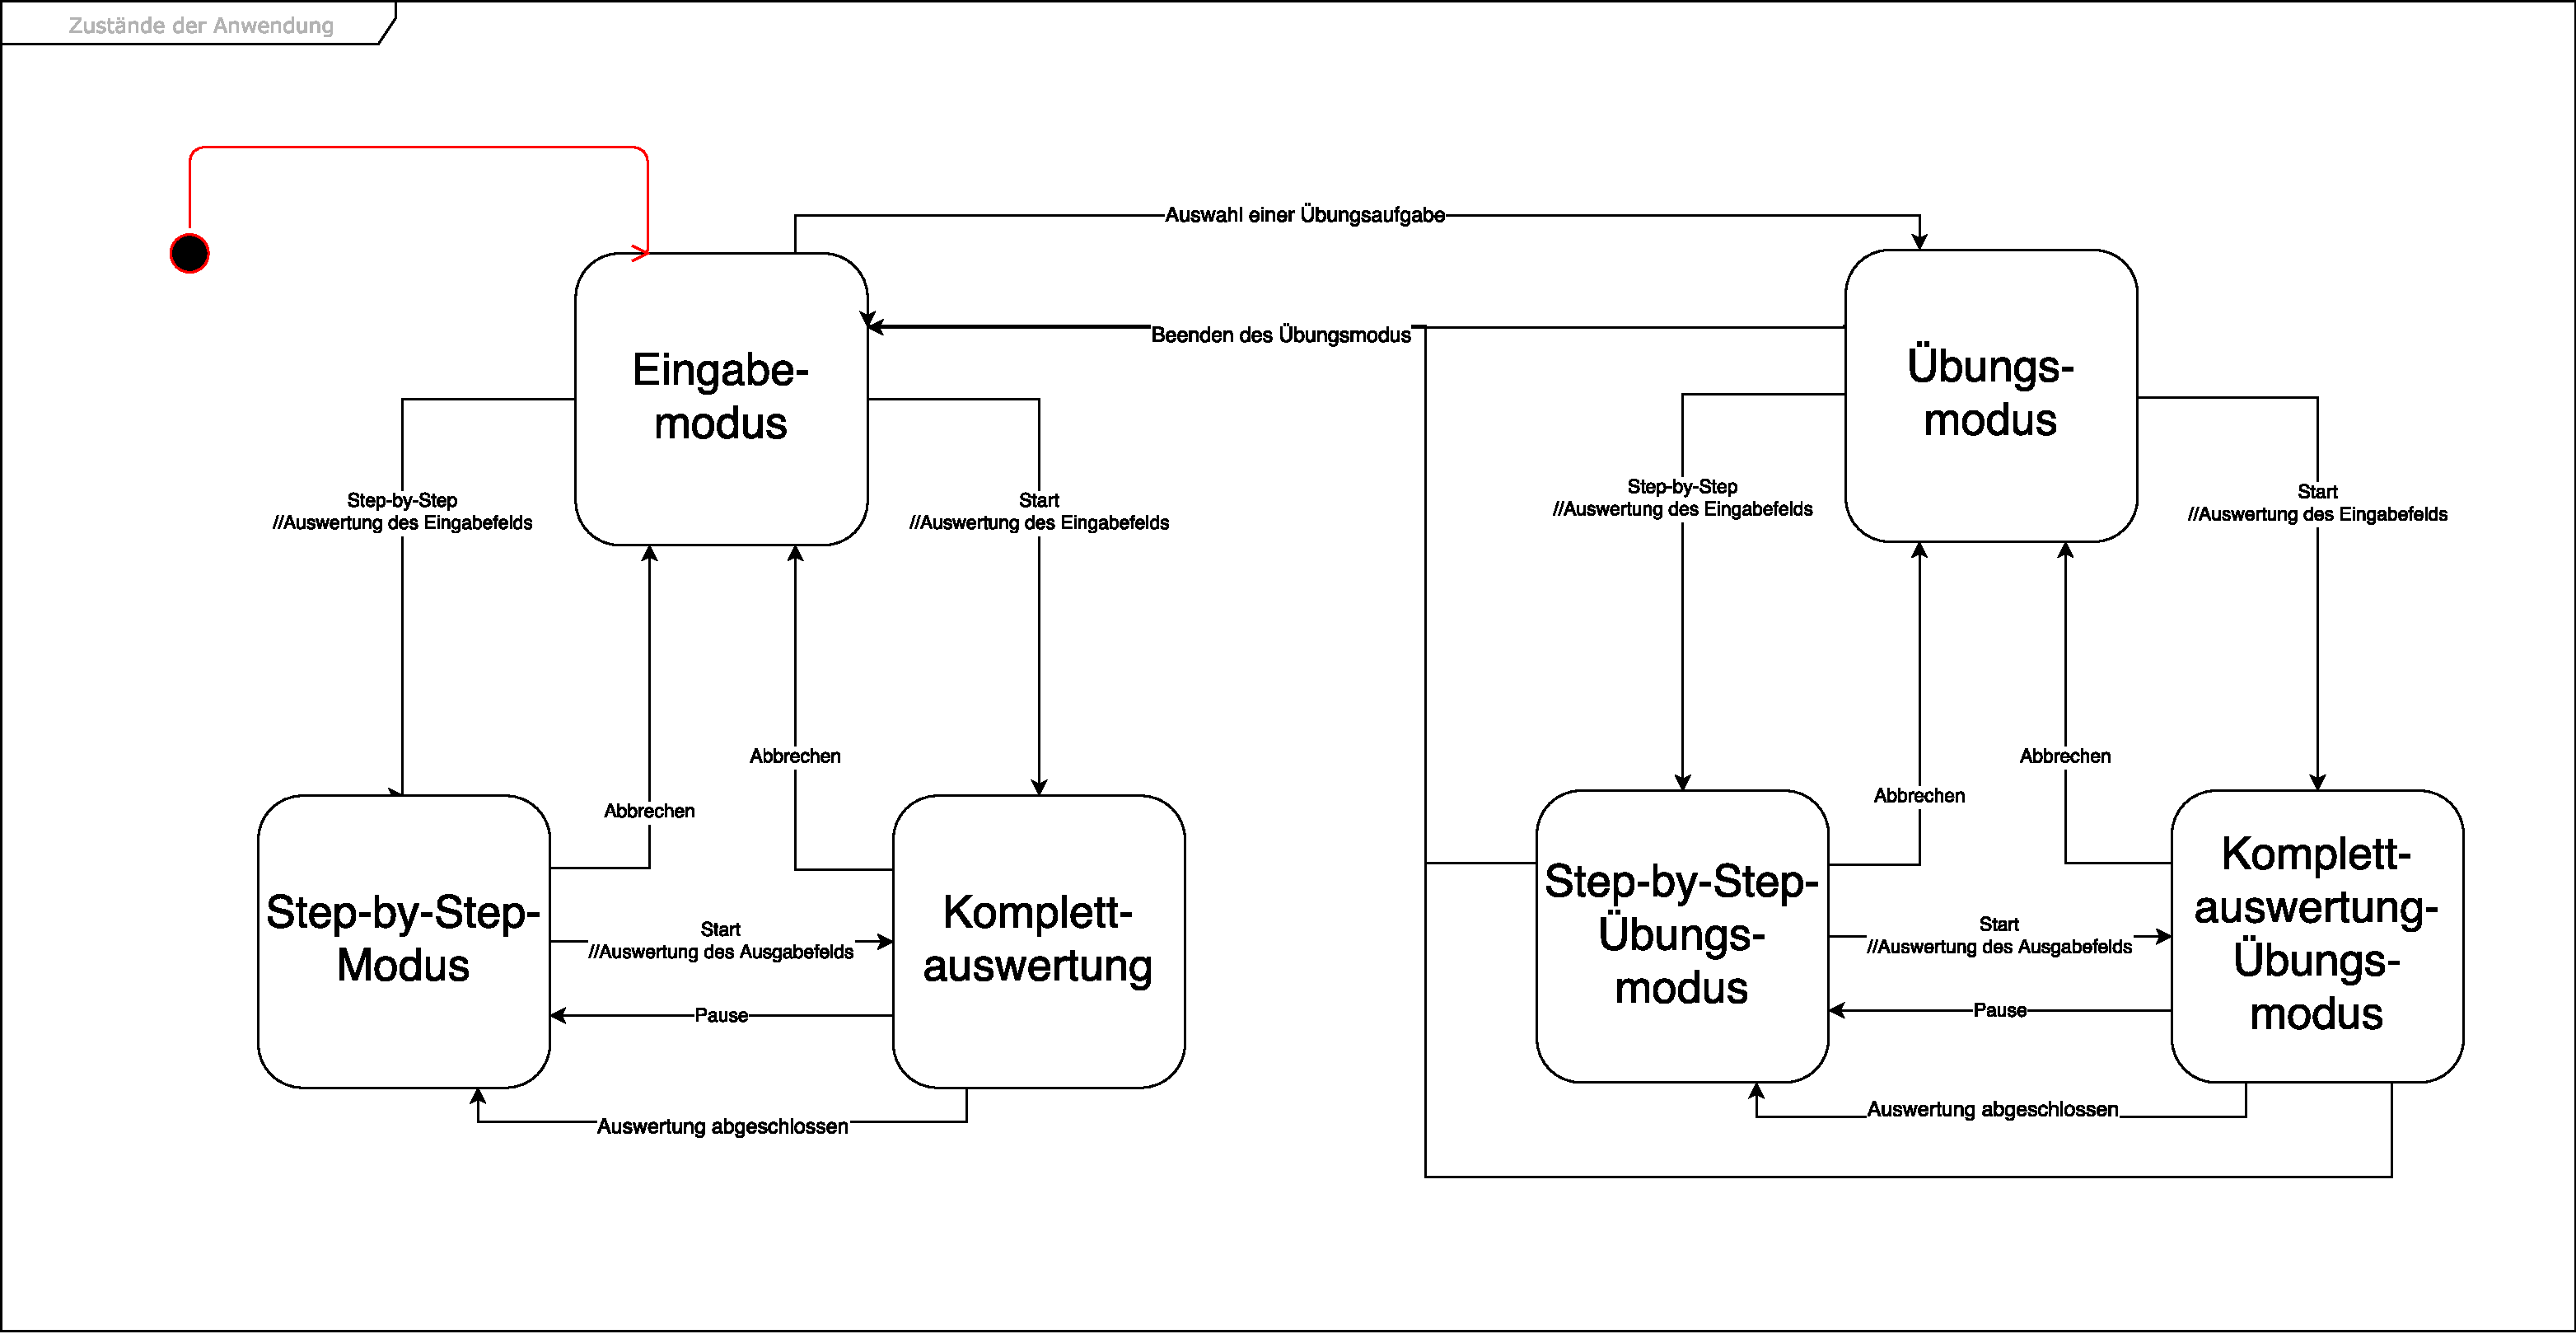
\includegraphics[width=\textwidth]{img/Zustandsautomat}
	\caption{\label{fig:state} Zustandsautomat der Anwendung}
\end{figure}

Die Anwendung kann sich in drei verschiedenen Zuständen befinden, wobei jeder Zustand ein Gegenstück im Übungsmodus besitzt. 
%TODO verlinken vom Übunsgmodus
Der Übungsmodus wird durch Auswahl einer Übungsaufgabe betreten und durch Beendigung des Übungsmodus verlassen.\\
Beim Start der Anwendung befindet sich der Nutzer im Eingabemodus. In diesem Modus kann der Nutzer einen \gls{lt} in das Eingabefeld eingeben. 
Durch drücken des Step-by-Step oder Start Knopfes (\cref{fig:actionButtons}) gelangt der Nutzer in den jeweiligen Auswertungsmodus und es beginnt die Auswertung des eingegebenen \glslink{lt}{$\lambda$-Terms}. 
Zeitgleich wird das Eingabefeld deaktiviert. Wenn noch Ausgaben einer früheren Auswertung im Ausgabefeld stehen, werden diese gelöscht.\\ 
Durch Drücken des Start oder Pause Knopfes kann der Nutzer zwischen den entsprechenden Auswertungsmodi wechseln. 
Insbesondere wird beim Wechsel von Step-by-Step-Modus zur Komplettauswertung der zuletzt ausgegebene \gls{lt} des Ausgabefeldes weiter ausgewertet.
Die Auswertungsmodi können erst durch das Drücken des Abbrechen Knopfes verlassen werden. Es erscheint eine entsprechende Ausgabe in Ausgabefeld. Erst jetzt kann der Nutzer neue Eingaben im Eingabefeld auswerten lassen.


%%%%%%%%%%%
\section{Tests}

\test{Komplettauswertung}{tst:complete}
\tests{fnc:ed}
\tests{fnc:completereduce}
\tests{fnc:live}
\tests{fnc:nr}

\teststep{Nutzer "Ben Fielder" hat einen Browser geöffnet.}
{Ben navigiert zur URL des Wavelength-Projekts.}
{Die IDE öffnet sich wie in Abbildung~\ref{img:start}.}

\teststep{Die IDE ist bereit.}
{Ben gibt in das Eingabefeld im oberen Teil des Fensters einen gültigen \gls{lt},
dessen Reduktion durch die \gls{nr} terminiert, ein.
Hierbei verwendet er zur Navigation des Textfelds die Pfeiltasten und die
"Home"- und "End"-Tasten seiner Tastatur und die Tastenkombination "Strg+Z", um eine
versehentliche Änderung rückgängig zu machen.}
{Das Textfeld verhält sich wie erwartet.}

\teststep{Der \gls{lt} wurde eingegeben.}
{Ben überprüft, dass als Darstellungsmodus die Unicode-Darstellung, als Reduktionsordnung
die \gls{nr} und als Ausgabeumfang die volle Ausgabe ausgewählt sind.}
{Die IDE ist mit den korrekten Standardeinstellungen initialisiert.}

\teststep{Alle Einstellungen sind korrekt.}
{Ben betätigt den "Start"-Knopf}
{Das Ausgabefeld füllt sich graduell mit den Zwischenschritten, welche gemäß der \gls{nr} auftreten.
Zum Schluss wird die Normalform des eingangs eingegebenen Terms ausgegeben.}

\test{Schritt-für-Schritt-Auswertung}{tst:steps}
\tests{fnc:awsstrats}
\tests{fnc:cbn}
\tests{fnc:cbv}
\tests{fnc:ao}
\tests{fnc:steps}
% fehlt: \tests{fnc:interactive}

\teststep{Benutzer "Donald Knuth" befindet sich auf der Wavelength-Seite.}
{Er gibt einen syntaktisch korrekten \gls{lt} in das Eingabefeld ein und betätigt
die "Step-by-Step"-Schaltfläche.}
{Der eingegebene Term wird in das Darstellungsfeld übernommen und die Vor- und
Zurück-Schaltflächen werden aktiv. Im Term wird der nächste $\beta$-Reduktionsschritt
gemäß der \glslink{nr}{normalen Reduktionsordnung} markiert.}

\teststep{Die IDE ist bereit für die Schritt-für-Schritt-Auswertung.}
{Don betätigt die Vor-Schaltfläche.}
{Das Resultat der markierten Reduktion erscheint als neue Zeile im Darstellungsfeld.
Die Markierungen der vorherigen Zeile werden entfernt, stattdessen wird in der neuen
aktuellen Zeile der nächste Reduktionsschritt markiert.}

\teststep{Die IDE ist bereit für die nächste Eingabe.}
{Don betätigt die Zurück-Schaltfläche.}
{Der zweite Reduktionsschritt wird aus dem Darstellungsfeld entfernt. Die Markierungen
auf dem Ausgangsschritt erscheinen wieder.}

\teststep{Die IDE ist bereit für die nächste Eingabe.}
{Don schwebt mit der Maus über einem nicht markierten, zu einem \gls{redex} gehörenden
$\lambda$-Symbol in der aktiven Zeile im Darstellungsfeld.}
{Die alten Markierungen verschwinden. Neue Markierungen für den \gls{redex}, über dem
sich die Maus befindet, erscheinen.}

\teststep{Der Mauszeiger befindet sich über einem Redex.}
{Don bewegt die Maus von diesem Redex weg.}
{Die Markierungen verschwinden und die Markierungen gemäß der \glslink{nr}{normalen Reduktionsordnung}
werden wieder angezeigt.}

\teststep{Die IDE ist bereit für die nächste Eingabe.}
{Don klickt mit der Maus auf ein zu einem \gls{redex} gehörendes $\lambda$-Symbol.}
{Es erscheint eine neue Zeile im Darstellungsfeld, die das Ergebnis der angeklickten
Reduktion enthält. Die Markierungen in der darüberliegenden Zeile werden ausgeblendet
und in der neuen Zeile erscheinen die Markierungen gemäß der ausgewählten
Reduktionsordnung.}

\teststep{Die IDE ist bereit für die nächste Eingabe.}
{Don wählt das Drop-down-Menü für die Reduktionsordnung an. Er wählt "\gls{cbn}".}
{Die Markierungen für die vorher ausgewählte Reduktionsordnung werden ausgeblendet.
Stattdessen wird der nächste Schritt gemäß \gls{cbn} angezeigt.}

\teststep{Die IDE ist bereit für die nächste Eingabe.}
{Don betätigt die Vor-Schaltfläche.}
{Das Resultat der markierten Reduktion (gemäß \gls{cbn}) erscheint als neue Zeile im Darstellungsfeld.
Die Markierungen der vorherigen Zeile werden entfernt, stattdessen wird in der neuen
aktuellen Zeile der nächste Reduktionsschritt markiert.}

\teststep{Die IDE ist bereit für die nächste Eingabe.}
{Don wählt das Drop-down-Menü für die Reduktionsordnung an. Er wählt "\gls{cbv}".}
{Die Markierungen für die vorher ausgewählte Reduktionsordnung werden ausgeblendet.
Stattdessen wird der nächste Schritt gemäß \gls{cbv} angezeigt.}

\teststep{Die IDE ist bereit für die nächste Eingabe.}
{Don betätigt die Vor-Schaltfläche.}
{Das Resultat der markierten Reduktion (gemäß \gls{cbv}) erscheint als neue Zeile im Darstellungsfeld.
Die Markierungen der vorherigen Zeile werden entfernt, stattdessen wird in der neuen
aktuellen Zeile der nächste Reduktionsschritt markiert.}

\teststep{Die IDE ist bereit für die nächste Eingabe.}
{Don wählt das Drop-down-Menü für die Reduktionsordnung an. Er wählt "\gls{ao}".}
{Die Markierungen für die vorher ausgewählte Reduktionsordnung werden ausgeblendet.
Stattdessen wird der nächste Schritt gemäß \gls{ao} angezeigt.}

\teststep{Die IDE ist bereit für die nächste Eingabe.}
{Don betätigt die Vor-Schaltfläche.}
{Das Resultat der markierten Reduktion (gemäß \gls{ao}) erscheint als neue Zeile im Darstellungsfeld.
Die Markierungen der vorherigen Zeile werden entfernt, stattdessen wird in der neuen
aktuellen Zeile der nächste Reduktionsschritt markiert.}

\test{Erstellen vom Permalinks}{tst:perma}
\tests{fnc:perma}
\tests{fnc:steps}

\teststep{Benutzer "Edsger Dijkstra" befindet sich auf der Wavelength-Seite.}
{Edsger gibt einen gültigen \gls{lt} in die Software ein, wählt eine Reduktionsordnung und einen
Darstellungsmodus aus, begibt sich in den Schritt-für-Schritt-Modus und durchläuft einige
Schritte der Auswertung.}
{Die Anwendung verhält sich wie spezifiziert.}

\teststep{Die IDE ist bereit für die nächste Aktion.}
{Edsger wählt die "Share"-Schaltfläche im unteren Bereich der Anwendung an.}
{Neben der Schaltfläche erscheint eine URL wie in Abbildung~\ref{img:share}
abgebildet.}

\teststep{Edsger hat die URL in seine Zwischenablage kopiert.}
{Edsger wählt die URL in einem neuen Browserfenster an.}
{Die IDE öffnet sich im neuen Fenster und befindet sich im gleichen Zustand wie im
alten Fenster.}

\teststep{Die IDE ist im neuen Fenster geöffnet.}
{Edsger wählt die Zurück-Schaltfläche.}
{Der letzte, im alten Browserfenster durchgeführte, Schritt wird im neuen Browserfenster
rückgängig gemacht.}

\test{Übungsmodus}{tst:ex}
\tests{fnc:ex}

\teststep{Benutzerin "Ada Lovelace" befindet sich auf der Wavelength-Seite.}
{Ada wählt im Menü (vgl. \cref{fig:exerciseMode}) eine Übungsaufgabe aus.}
{Der Übungsmodus wird aktiviert. 
 Das Eingabefeld wird aufgeteilt in ein schmaleres Eingabefeld und ein Aufgabenfeld.
 Im Aufgabenfeld erscheint eine Beschreibung der gewählten \gls{ex}.
 Der "Beenden"- und der "zeige Lösung"-Knopf erscheinen.}

\teststep{Die IDE ist bereit für die nächste Aktion.}
{Ada gibt eine syntaktisch korrekte Lösung ein, die kein korrektes Ergebnis liefert.
 Ada drückt den "Start"-Knopf.}
{Die IDE wertet die Eingabe wie spezifiziert aus.
 Es wird angezeigt, dass die Lösung inkorrekt ist.}

\teststep{Die IDE ist bereit für die nächste Aktion.}
{Ada gibt die korrekte Lösung ein. Ada drückt den "Start"-Knopf.}
{Die IDE wertet die Eingabe wie spezifiziert aus.
 Es wird angezeigt, dass die Lösung korrekt ist.}
 
\teststep{Die IDE ist bereit für die nächste Aktion.}
{Ada wählt eine andere Übungsaufgabe aus.}
{Eingabe und Ausgabe werden entfernt.
Im Aufgabenfeld erscheinen eine Beschreibung der \gls{ex} und ein Stück Code.}

\teststep{Die IDE ist bereit für die nächste Aktion.}
{Ada vervollständigt den Code zu einer korrekten Lösung und durchläuft den Schritt-für-Schritt Modus komplett.}
{Die IDE verhält sich wie spezifiziert.
 Als letzter Schritt wird angezeigt, dass die eingegebene Lösung korrekt ist.}

\teststep{Die IDE ist bereit für die nächste Aktion}
{Ada drückt auf den "zeige Lösung"-Knopf.}
{Die Musterlösung wird im Aufgabenfeld eingefügt.
 Der "zeige Lösung"-Knopf wird zum "verberge Lösung"-Knopf.}

\teststep{Im Aufgabenfeld wird die Musterlösung angezeigt.}
{Ada kopiert die Musterlösung, überschreibt ihre Eingabe damit und drückt den "Start"-Knopf.}
{Die IDE verhält sich wie spezifiziert. 
 Als letzter Schritt wird angezeigt, dass die eingegebene Lösung korrekt ist.}
 
\teststep{Die IDE ist bereit für die nächste Aktion}
{Ada drückt auf den "verberge Lösung"-Knopf.}
{Die Musterlösung wird aus dem Aufgabenfeld entfernt.}
 
\teststep{Die IDE ist bereit für die nächste Aktion}
{Ada drückt den "Beenden"-Knopf.}
{Der Übungsmodus wird beendet, der "Beenden"-Knopf verschwindet, Eingabe und Ausgabe werden entfernt.
 Das Aufgabenfeld wird entfernt.}

\test{Darstellungsformate}{tst:display}
\tests{fnc:display}
\tests{fnc:unicode}
\tests{fnc:tree}

\teststep{Benutzer "Richard Hamming" befindet sich auf der Wavelength-Seite.}
{Richard gibt einen syntaktisch korrekten \gls{lt} ein und drückt den "Start"-Knopf.}
{Der eingegebene \gls{lt} wird ausgewertet und im Unicode-Format im Ausgabefenster angezeigt.}

\teststep{Die IDE ist bereit für die nächste Aktion}
{Richard wählt im Dropdown-Menü (vgl. \cref{fig:display}) ein anderes Darstellungsformat und drückt den "Start"-Knopf.}
{Der eingegebene \gls{lt} wird ausgewertet und im gewählten Darstellungsformat wie spezifiziert dargestellt.}

\test{Export}{tst:output}
\tests{fnc:output}

\teststep{Benutzer "Robert Tarjan" befindet sich auf der Wavelength-Seite.}
{Robert gibt einen gültigen \gls{lt} ein und drückt auf den "Exportieren"-Knopf.}
{Es öffnet sich eine Liste mit allen Ausgabeformaten.}

\teststep{Die IDE erwartet die Auswahl eines Ausgabeformates.}
{Robert wählt ein beliebiges Ausgabeformat aus der Liste aus.}
{Die Liste mit den Ausgabeformaten verschwindet.
Es öffnet sich ein Fenster (vgl. \cref{fig:export}) mit der formatierten Eingabe.}

\teststep{Robert ist im Fenster mit der formatierten Eingabe.}
{Robert kopiert die formatierte Eingabe und schließt das Fenster.}
{Das Fenster mit der formatierten Eingabe verschwindet. 
 Die Eingabe aus dem ersten Schritt ist noch im Eingabefeld.}
 
\test{Namensbindung}{tst:bind}
\tests{fnc:bind}

\teststep{Benutzer "Haskell Curry" befindet sich auf der Wavelength-Seite.}
{Haskell gibt einen gültigen \gls{lt} ein und nennt ihn "curry".
 Haskell verwendet "curry" in einem weiteren gültigen \gls{lt} und drückt den "Start"-Knopf.}
{Die Eingabe wird gemäß Spezifikation ausgewertet (vgl. \gls{nb}).}

\teststep{Die IDE ist bereit für die nächste Aktion.}
{Haskell gibt einen gültigen \gls{lt} ein.
 Er benennt ihn mit einem gemäß Spezifikation (vgl. \gls{nb}) ungültigen Namen.
 Er drückt den "Start"-Knopf.}
{Es wird eine Fehlermeldung ausgegeben.
 Haskell wird darauf hingewiesen, dass er einen ungültigen Namen gewählt hat.}

\test{Auswahl der Ausgabelänge}{tst:selectsize}
\tests{fnc:selectsize}

\teststep{Benutzer "Wilhelm Ackermann" befindet sich auf der Wavelength-Seite.}
{Wilhelm gibt einen gültigen \gls{lt} ein und drückt auf den "Start"-Knopf. }
{Die Eingabe wird ausgewertet und nur das Ergebnis wird angezeigt (vgl. \gls{std}).}

\teststep{Die IDE ist bereit für die nächste Aktion.}
{Wilhelm wählt in der "output size"-Box eine andere Ausgabelänge aus (vgl. \ref{fig:outputOptions}) und drückt auf den "Start"-Knopf.}
{Die IDE verhält sich wie spezifiziert (vgl. \ref{fnc:selectsize}).}

\teststep{Die IDE ist bereit für die nächste Aktion.}
{Wilhelm wählt in der "display"-Box das Darstellungsformat "Tree" und drückt den "Start"-Knopf.}
{Die IDE verhält sich wie spezifiziert (vgl. \ref{fnc:completereduce}).
 Im Darstellungsfeld erscheint ein Syntaxbaum gemäß der ausgewählten Ausgabelänge (vgl. \ref{fnc:selectsize}).}
% Syntax:
% \test{Überschrift des Tests}{tst:label}
% \tests{fnc:label}
% \tests{nfc:label}
%
% \teststep{Stand}
% {Aktion}
% {Reaktion}
%
% \teststep{Stand}
% {Aktion}
% {Reaktion}
%
% ...

%%%%%%%%%%%%%
\pagebreak
\appendix

\section{Seitenentwürfe}

%TODO: resizing erklären
%TODO: einheitliche Benennung Button
%TODO: FA resizing
%TODO: wohin mit Kurzbeschreibung der Übungsaufgaben

% Hier ganz normale figures mit Bildern
Bei Aufruf der Website wird eine leere IDE angezeigt. Das obere Textfeld ist das Editorfeld, das untere ist das Ausgabefeld. Das Größenverhältnis der Felder kann mittels einer Schaltfläche angepasst werden.

\begin{figure}[H]
	\centering
	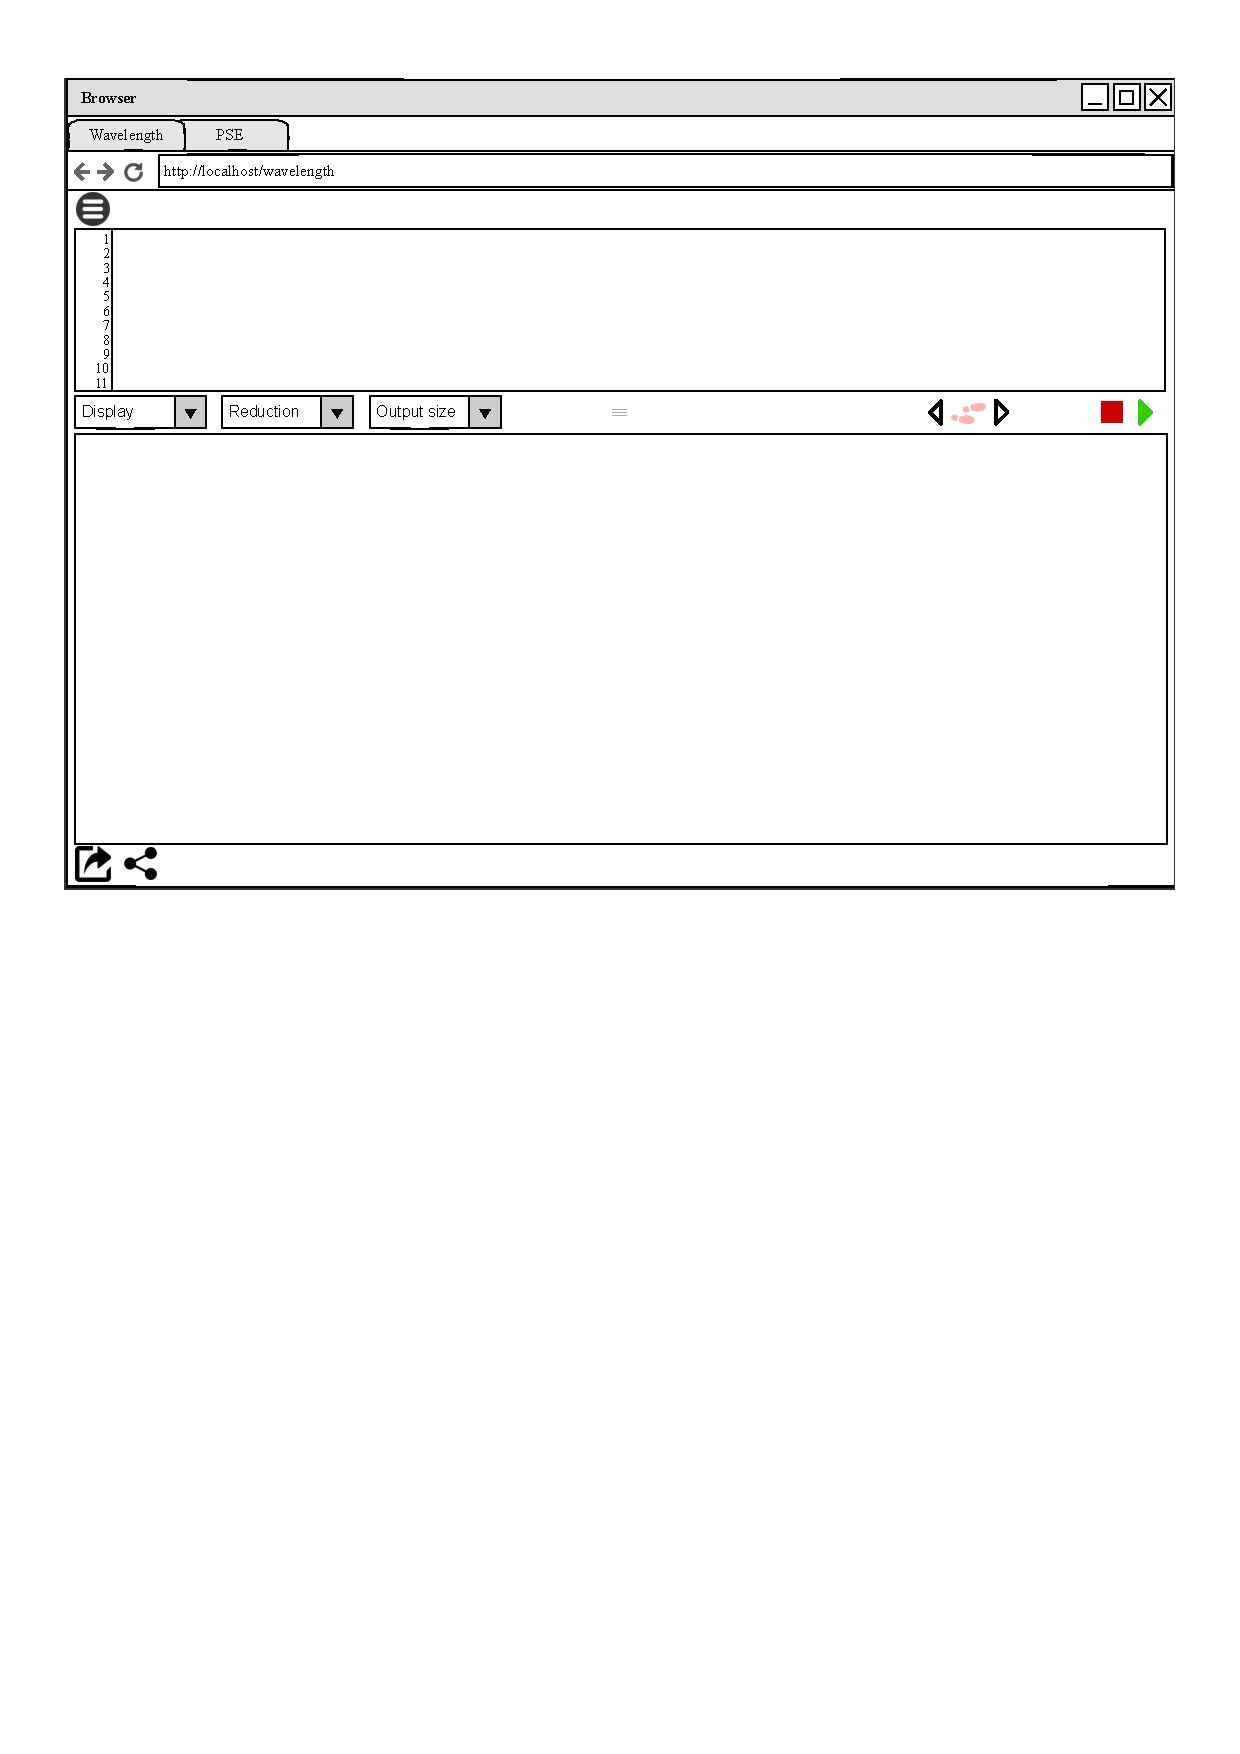
\includegraphics[width = \textwidth]{img/startseite}
	\caption{Die Startseite der IDE bei Aufruf der Website.} 
	\label{img:start}
\end{figure}


Der "Start"-Knopf löst die Auswertung zum Endergebnis aus. Durch Drücken des "Abbrechen"-Buttons wird die Auswertung abgebrochen. Bei Drücken der "Step-by-Step"-Schaltfläche wird die Schritt-für-Schritt-Auswertung gestartet, durch welche sich der Nutzer mit den beiden Knöpfen daneben navigieren kann.

\begin{figure}[H]
	\centering
	
\includegraphics{img/actionButton}
	\caption{\label{fig:actionButtons} Schritt-zurück, Step-by-Step-Modus, 
	Schritt-vor, Start und Abbrechen (von links nach rechts)}
\end{figure}



\begin{figure}[H]
	\centering
	
\includegraphics{img/pauseButton}
	\caption{Wurde die Auswertung mittels "Start" gestartet, erscheint ein "Pause"-Knopf um in den Step-by-Step-Modus wechseln zu können.}
\end{figure}


\begin{figure}[H]
	\begin{subfigure}[l]{0.25\textwidth}
	\centering
		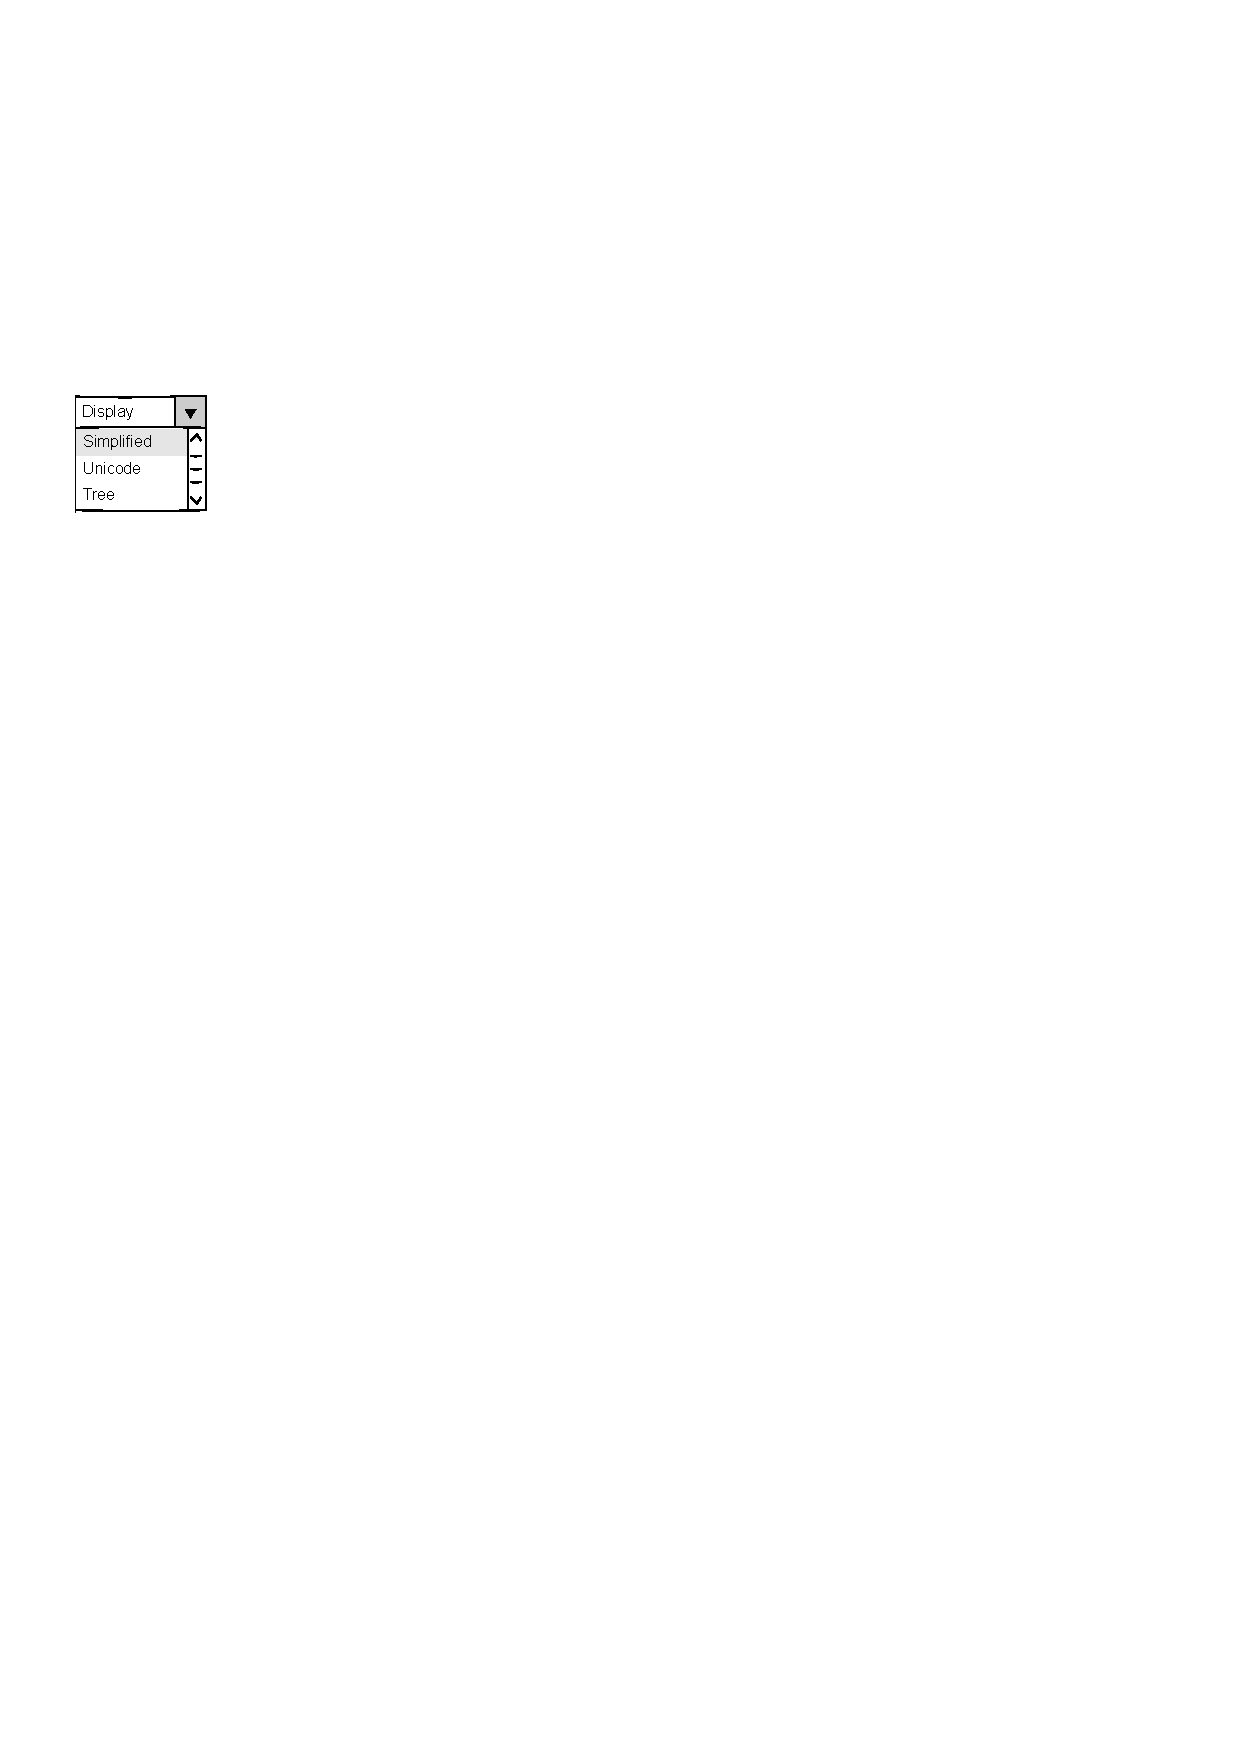
\includegraphics{img/displayMenu}
	\caption{\label{fig:display}Auswahl des Darstellungsformats}	
	\end{subfigure}
	\hspace*{\fill}
	\begin{subfigure}[m]{0.25\textwidth}
	\centering
		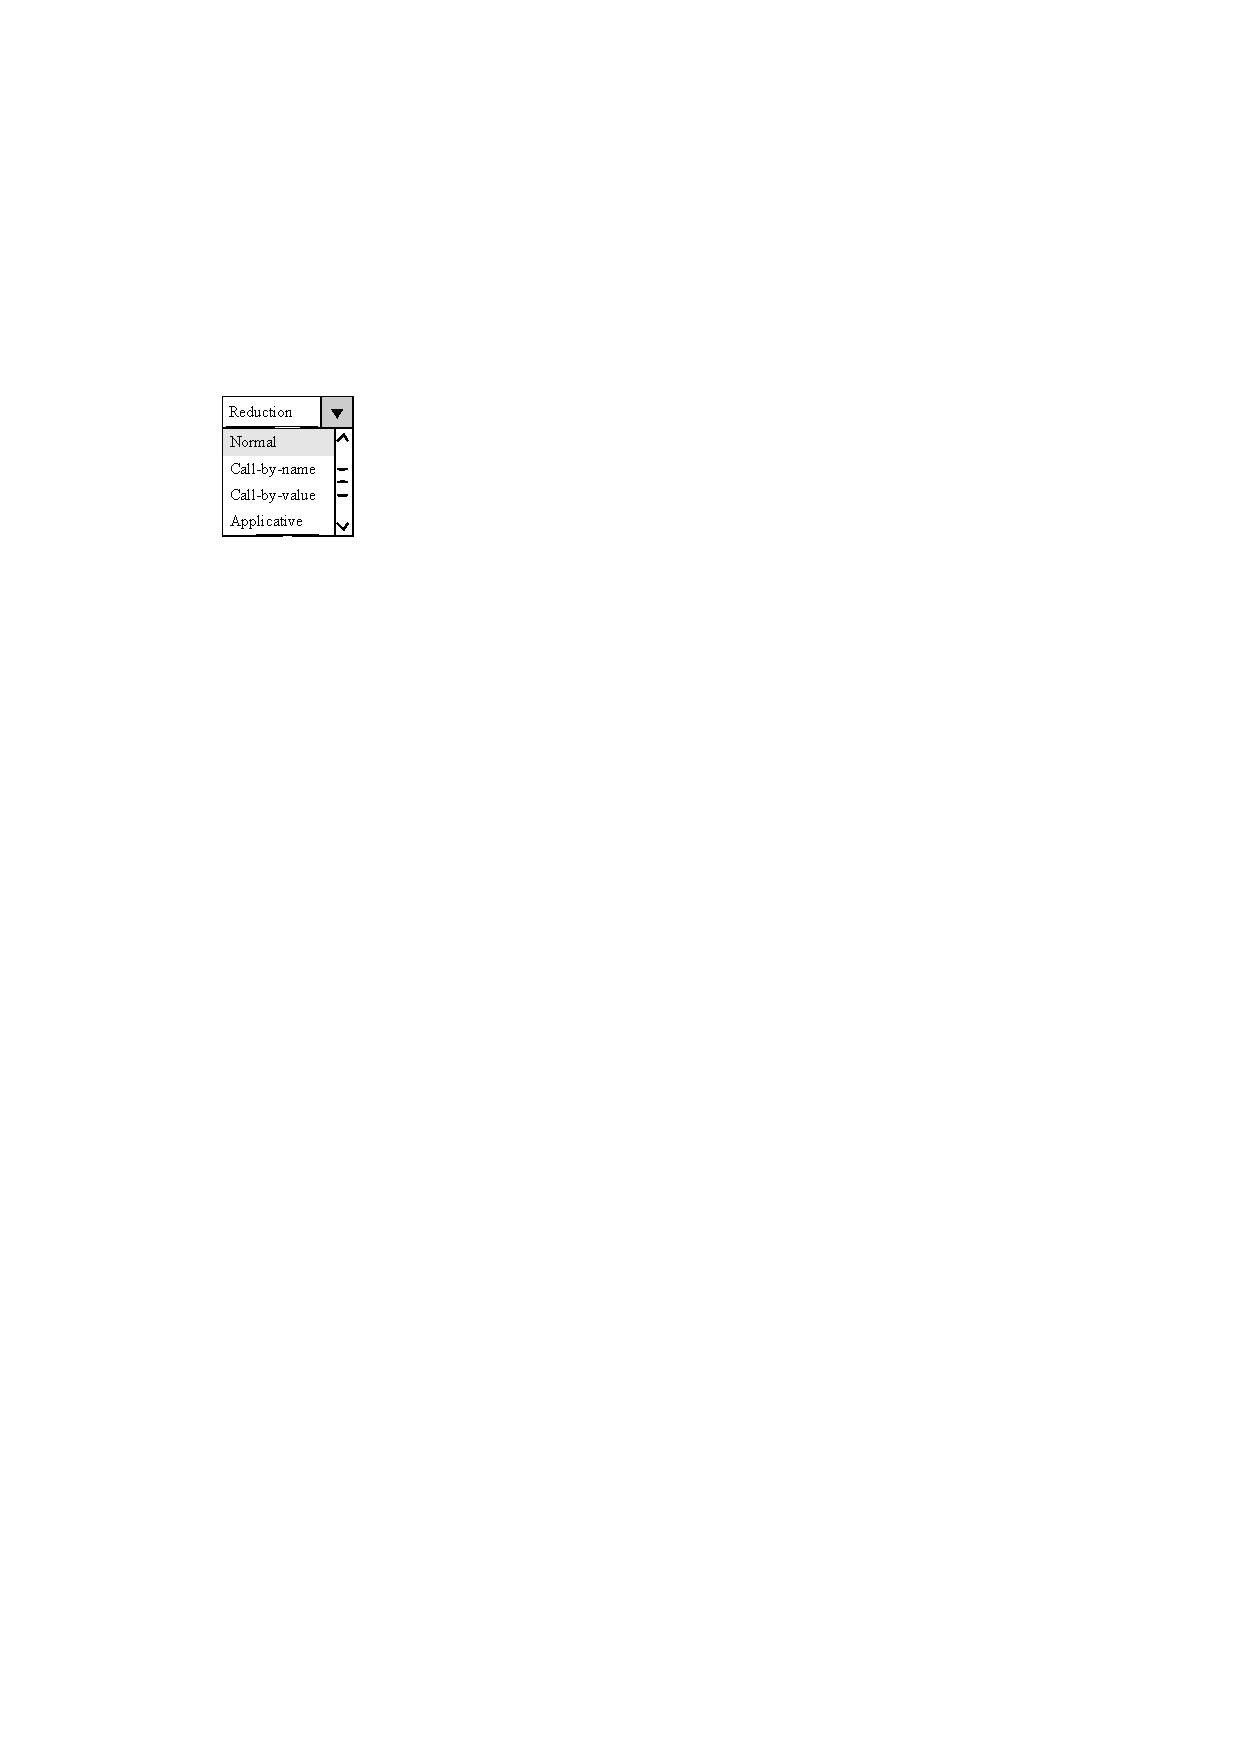
\includegraphics{img/reductionMenu}
	\caption{Auswahl der Auswertungsstrategie}
	\end{subfigure}
	\hspace*{\fill}
	\begin{subfigure}[r]{0.25\textwidth}
	\centering
		
\includegraphics{img/outputSizeMenu}
	\caption{Auswahl der Ausgabelänge}	
	\end{subfigure}
	\caption{\label{fig:outputOptions} Verschiedene Ausgabeoptionen können festgelegt werden.}
\end{figure}


\begin{figure}[H]
	\centering
	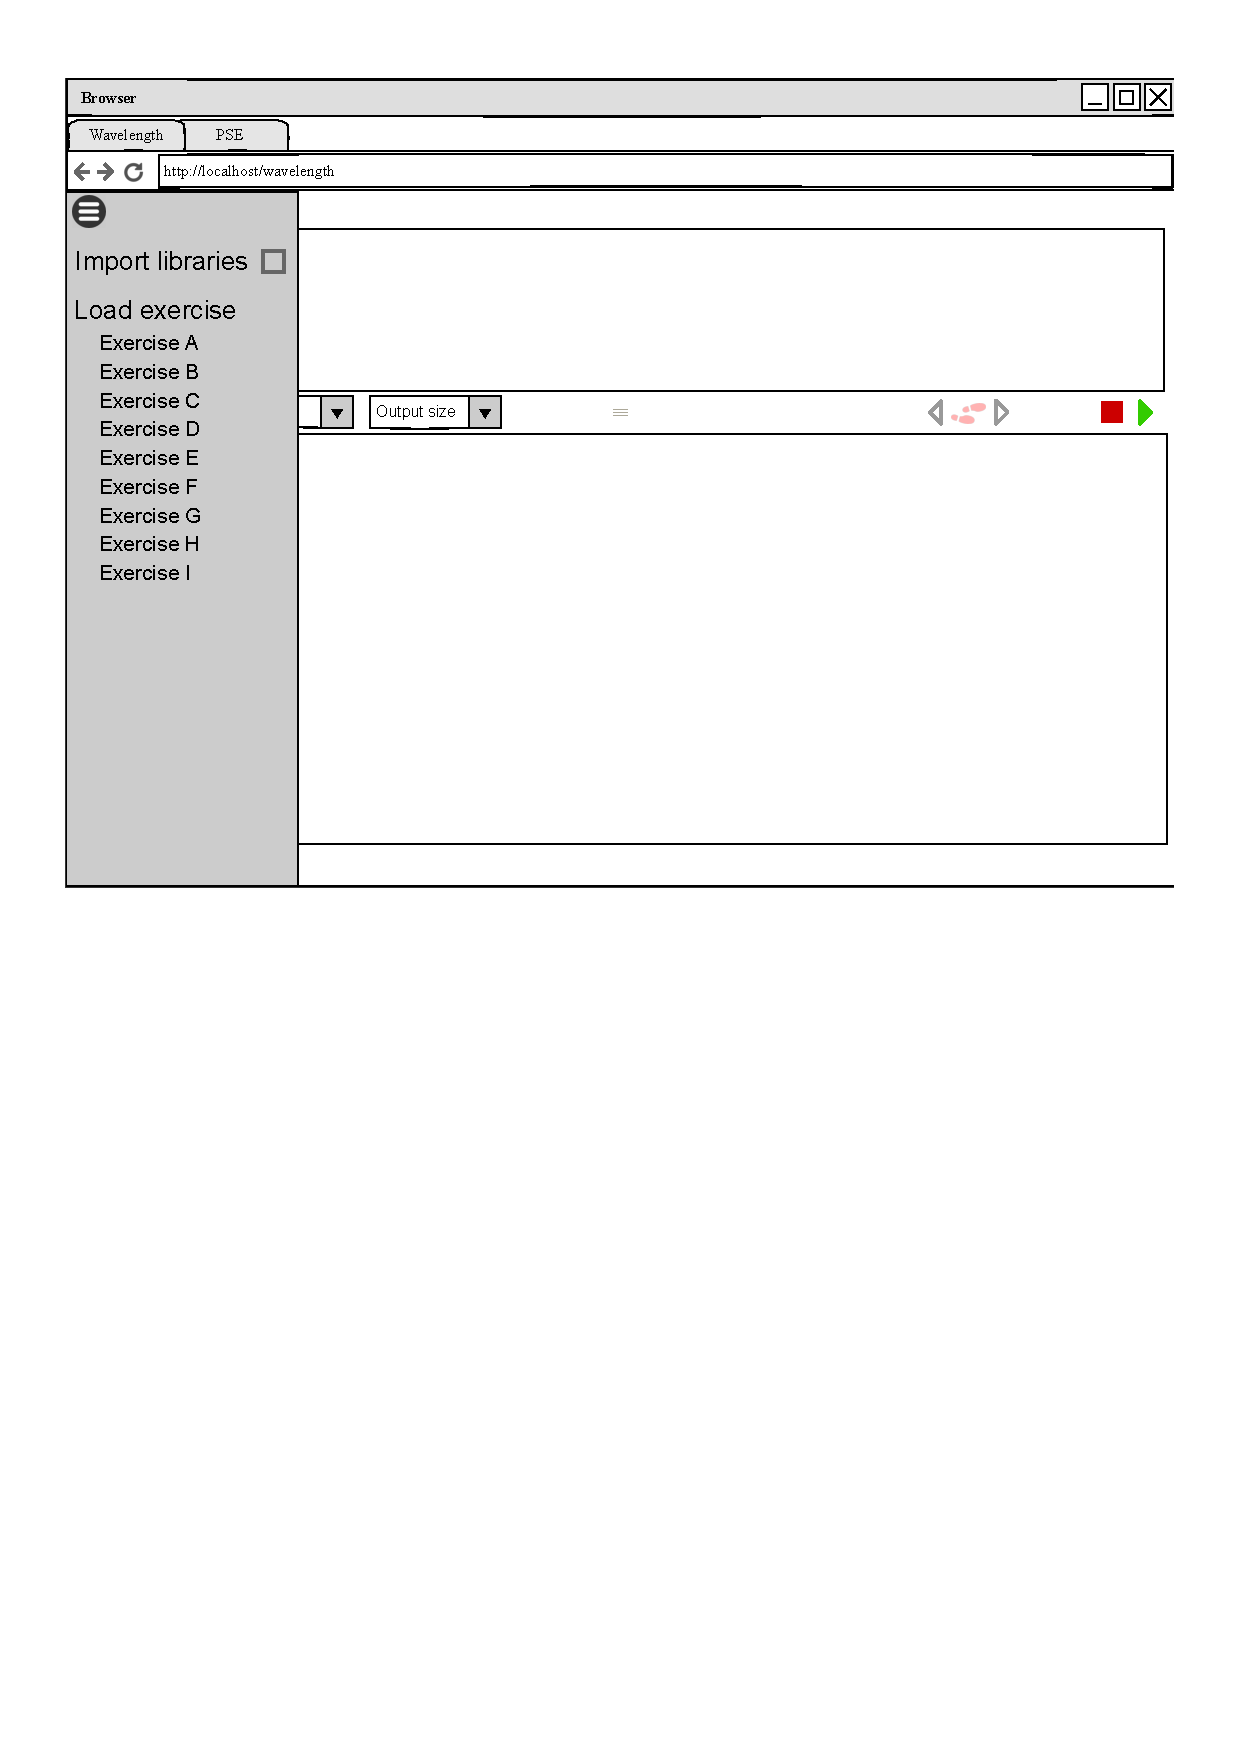
\includegraphics[width=\textwidth]{img/wavelength_exercise_menu_open}
	\caption{\label{fig:exmenu}Im Optionsmenü hat der Nutzer die Möglichkeit die Bibliothek einzubinden oder eine Übungsaufgabe auzuwählen.}
\end{figure}

\begin{figure}[H]
	\centering
	
\includegraphics[width=\textwidth]{img/wavelength_exerciseMode}
	\caption{\label{fig:exerciseMode} Wurde eine Übungsaufgabe ausgewählt, so wird die Aufgabenstellung in einem Textfeld angezeigt. Eventuell vorgegebene Eingaben werden in das Editorfenster geladen. Die Musterlösung der Aufgabe wird durch Klicken eines entsprechenden Button angezeigt werden. Mit Klick auf einen weiteren Button kann der Übungsmodus beendet werden.}
\end{figure}


\begin{figure}[H]
	\centering
	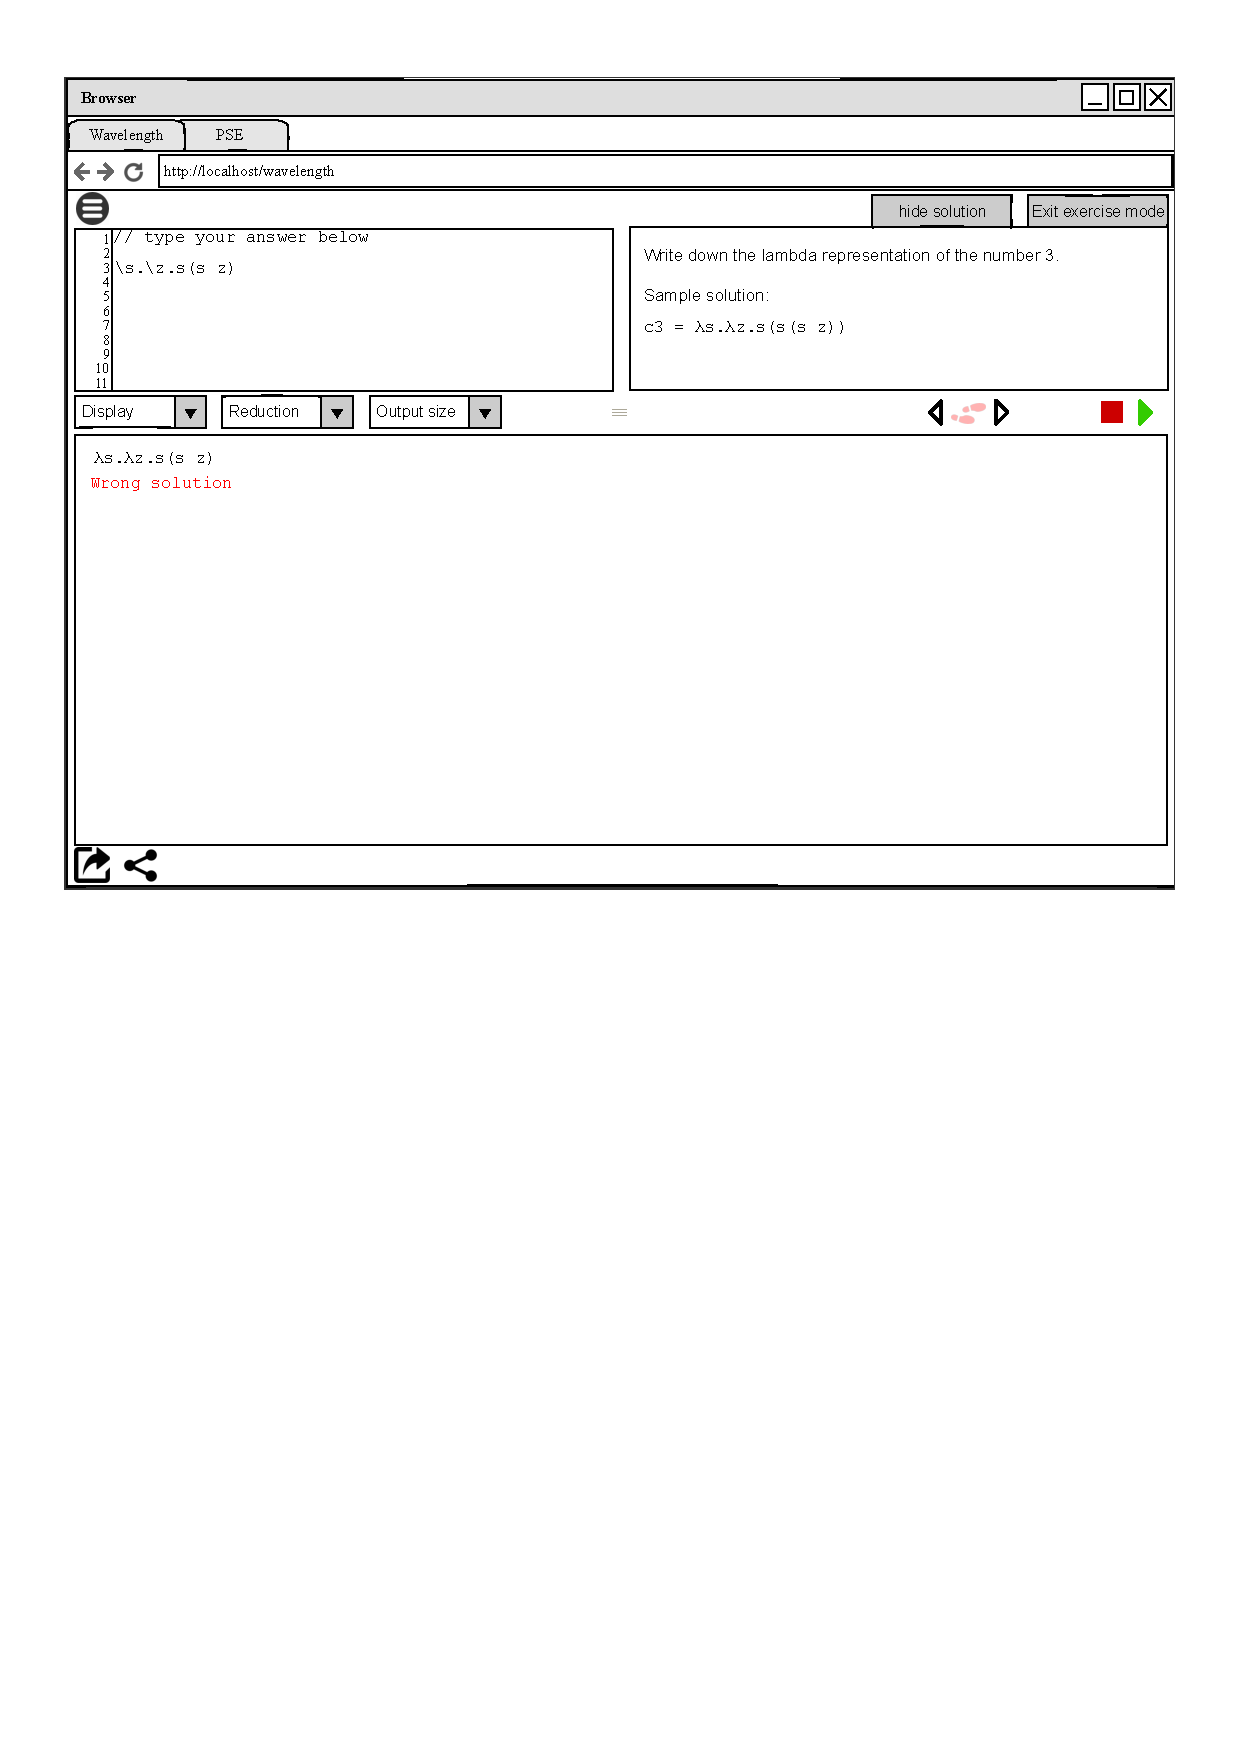
\includegraphics[width=\textwidth]{img/exerciseModeSolutionCheck}
	\caption{\label{fig:solutionCheck}Lässt der Nutzer seine Eingabe prüfen, so wird im Ausgabefeld angezeigt, ob diese korrekt ist.}
\end{figure}


\begin{figure}[H]
	\centering
	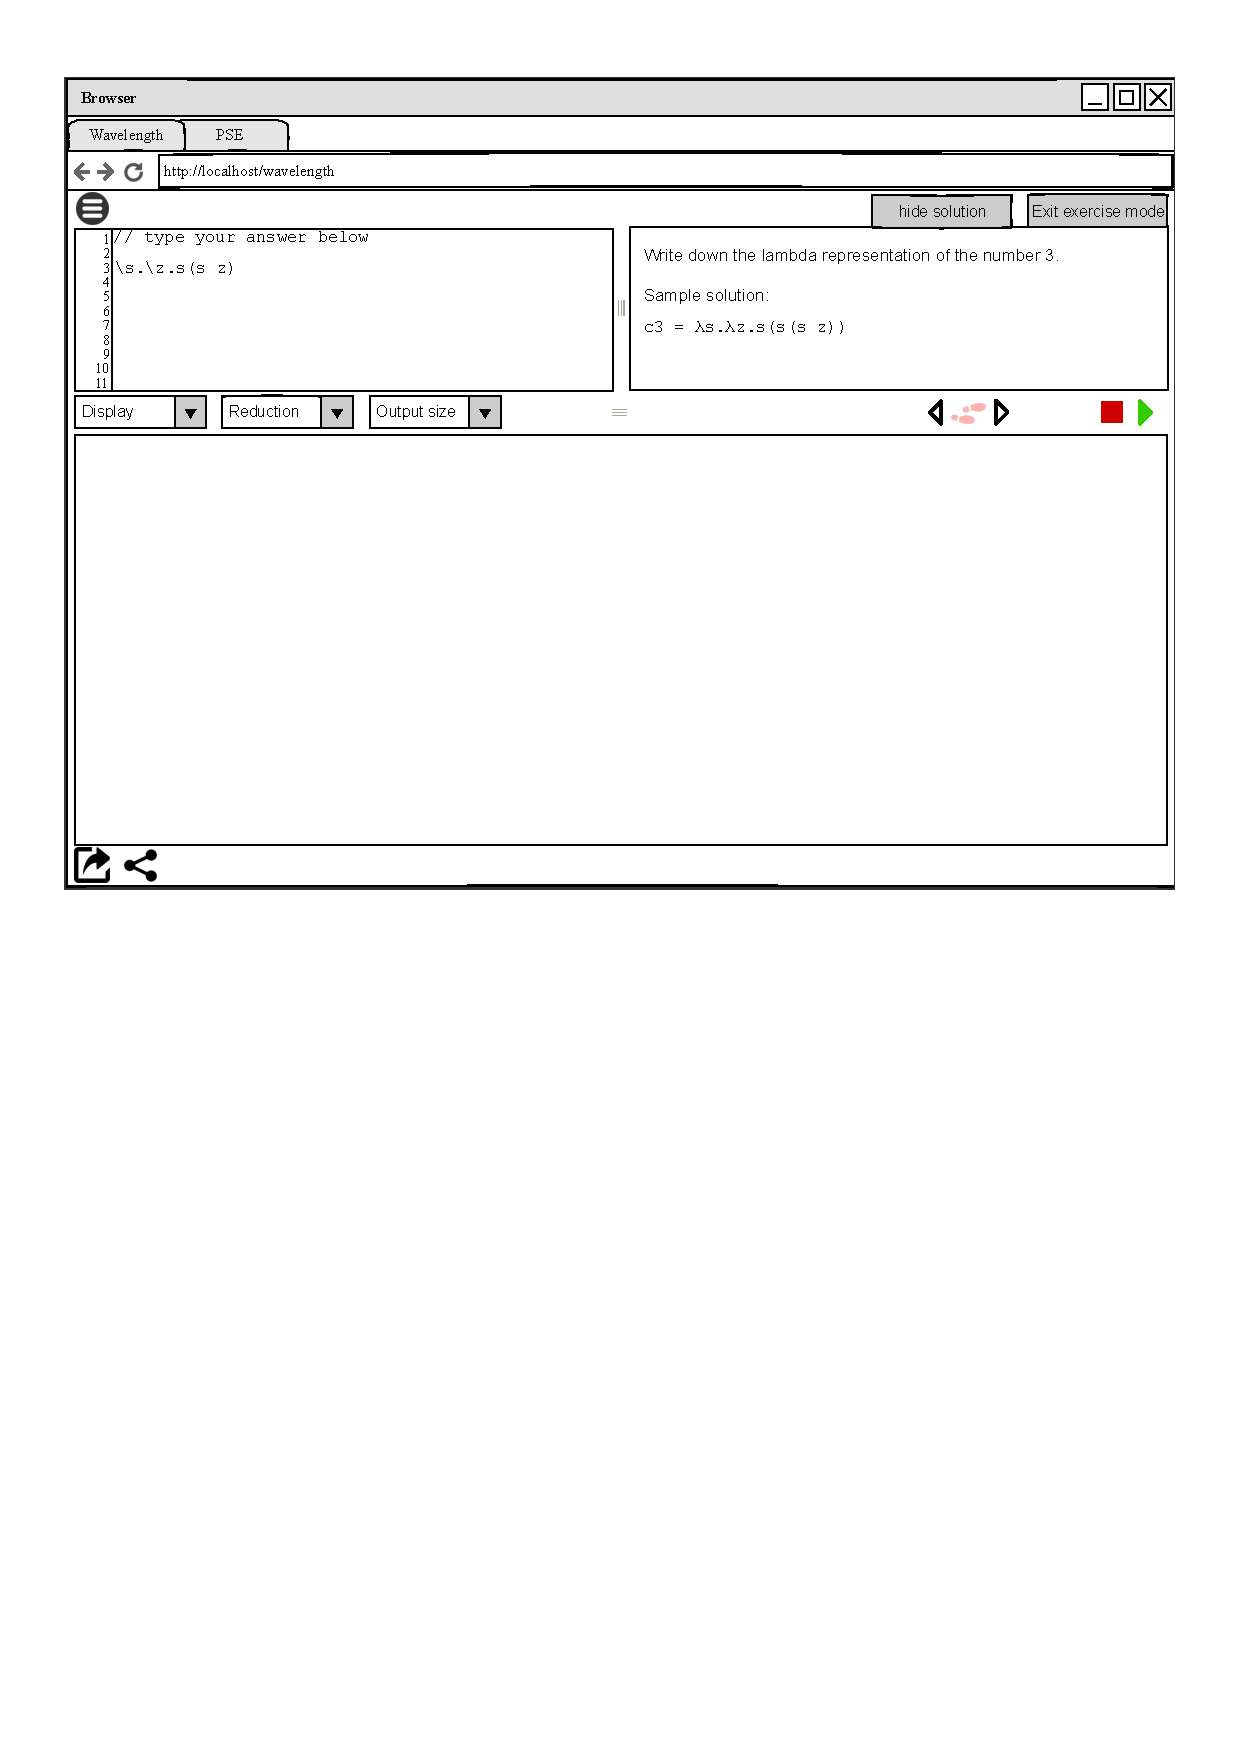
\includegraphics[width=\textwidth]{img/exerciseModeSolution}
	\caption{\label{fig:showSolution}Wird die Musterlösung angezeigt, so hat der Nutzer die Möglichkeit diese auch wieder auszublenden.}
\end{figure}


\begin{figure}[H]
	\centering
	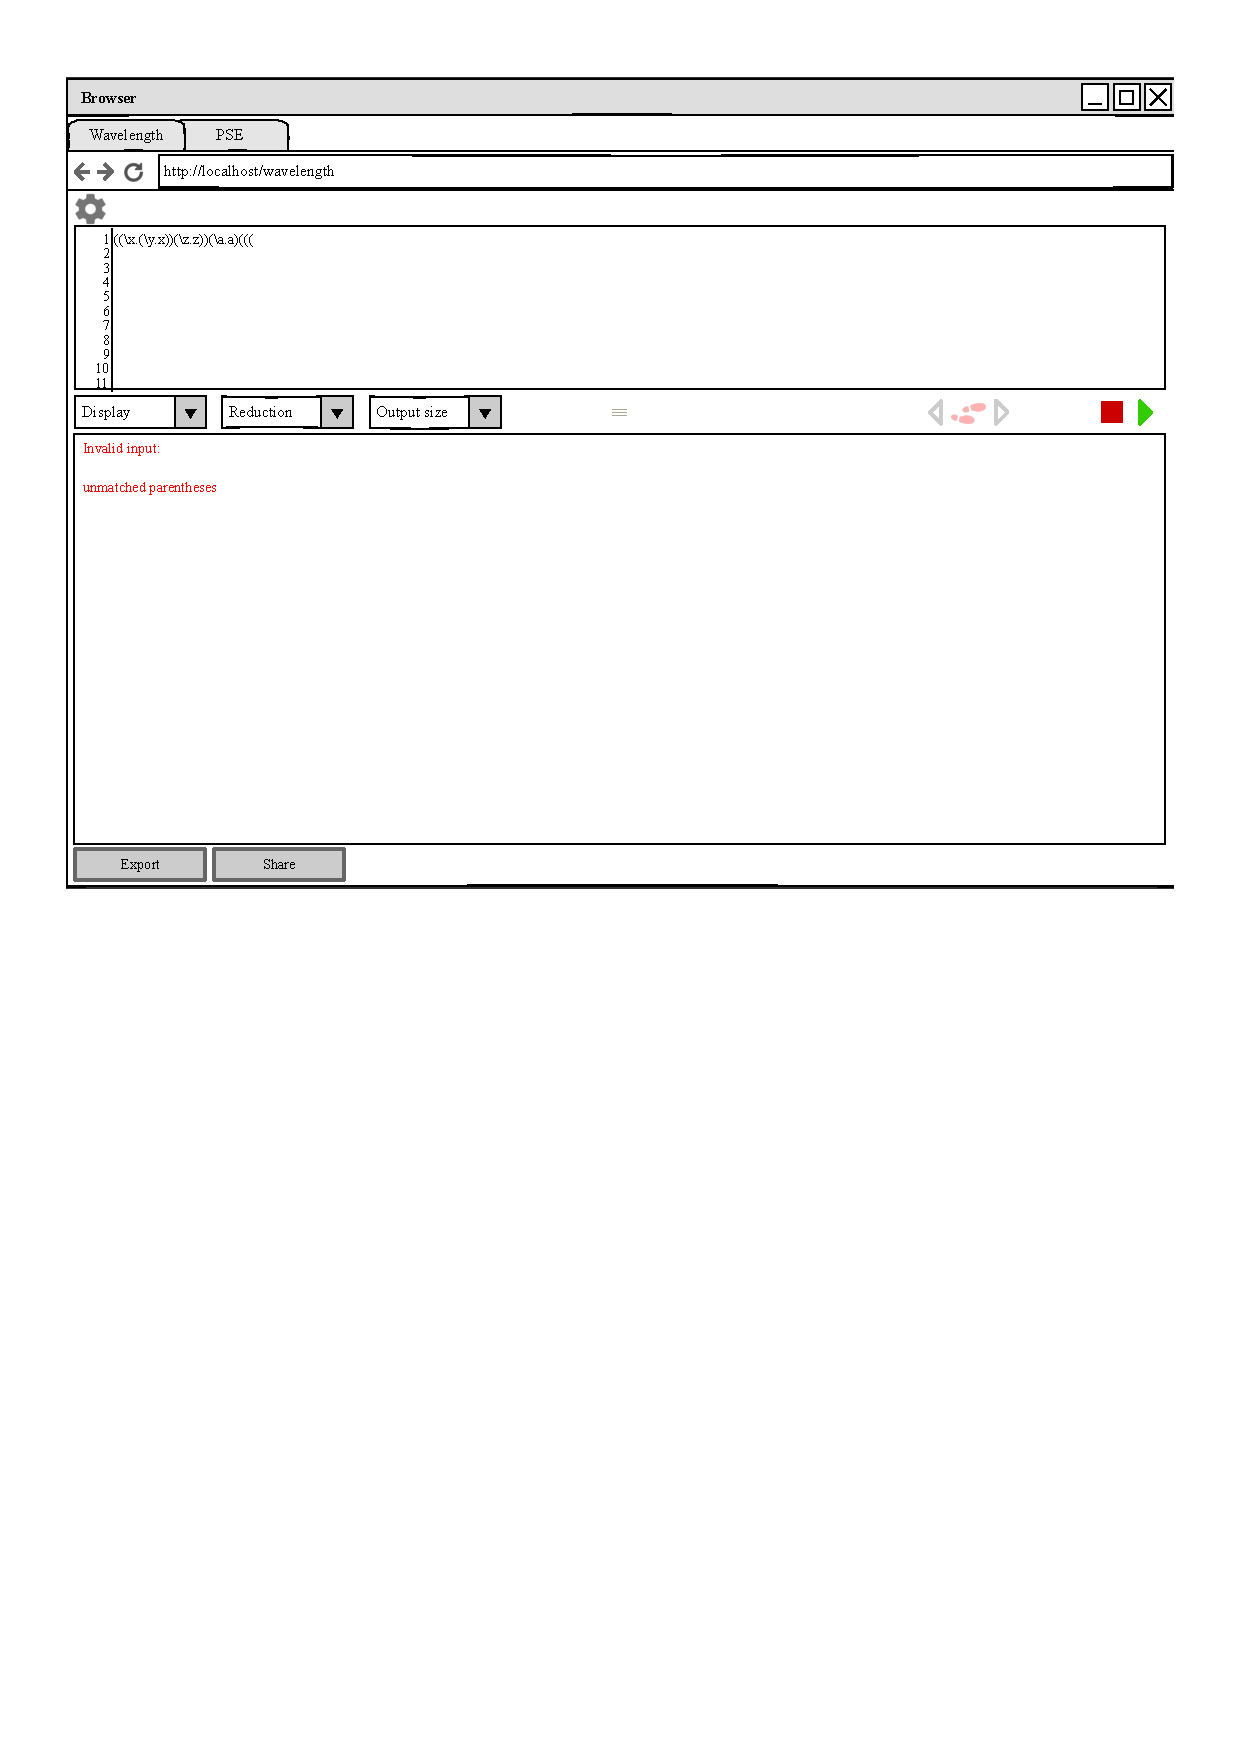
\includegraphics[width=\textwidth]{img/fehlerausgabe}
	\caption{Bei fehlerhafter Eingabe wird eine Fehlermeldung im Ausgabefenster ausgegeben.
}
\end{figure}



\begin{figure}[H]
	\begin{subfigure}{0.25\textwidth}
		\centering
		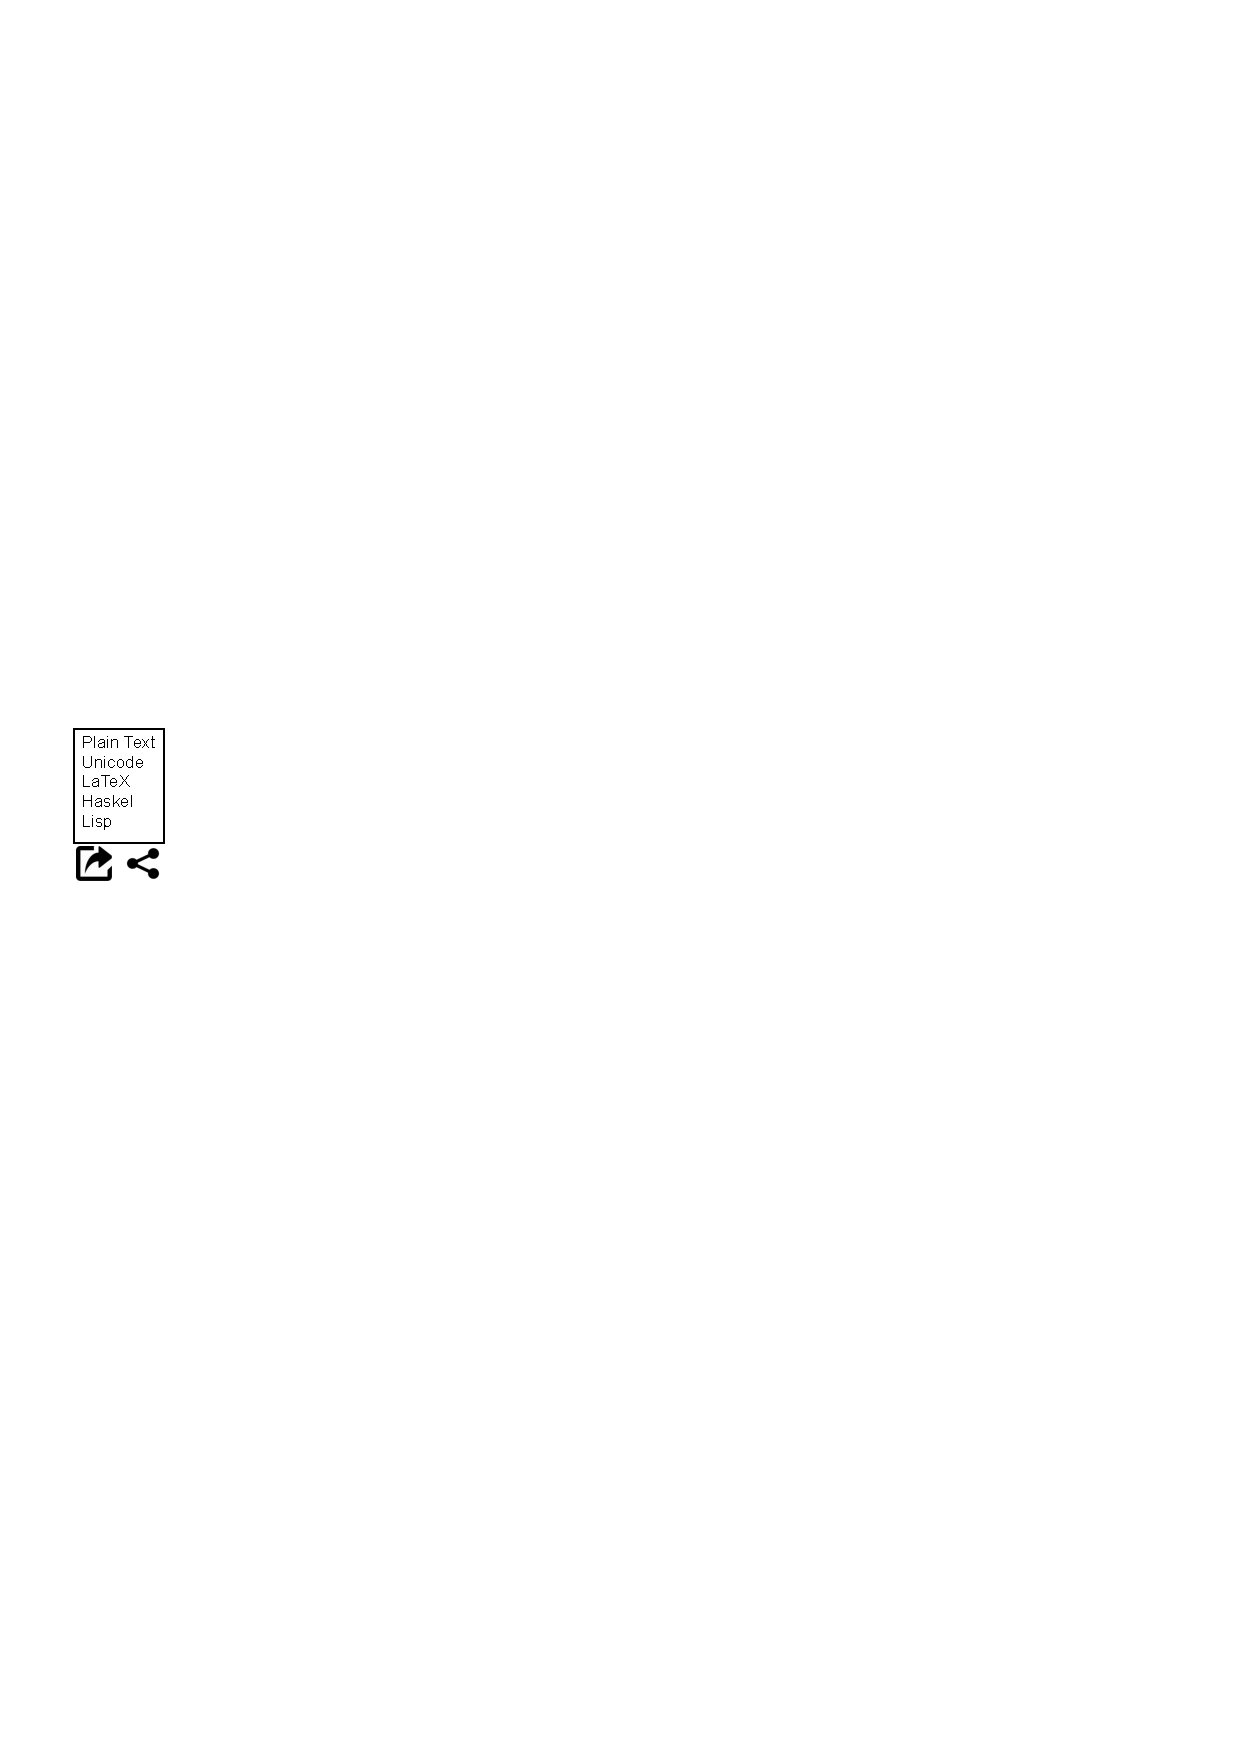
\includegraphics{img/exportMenu}
	\end{subfigure}
	\begin{subfigure}{0.75\textwidth}
		\centering
		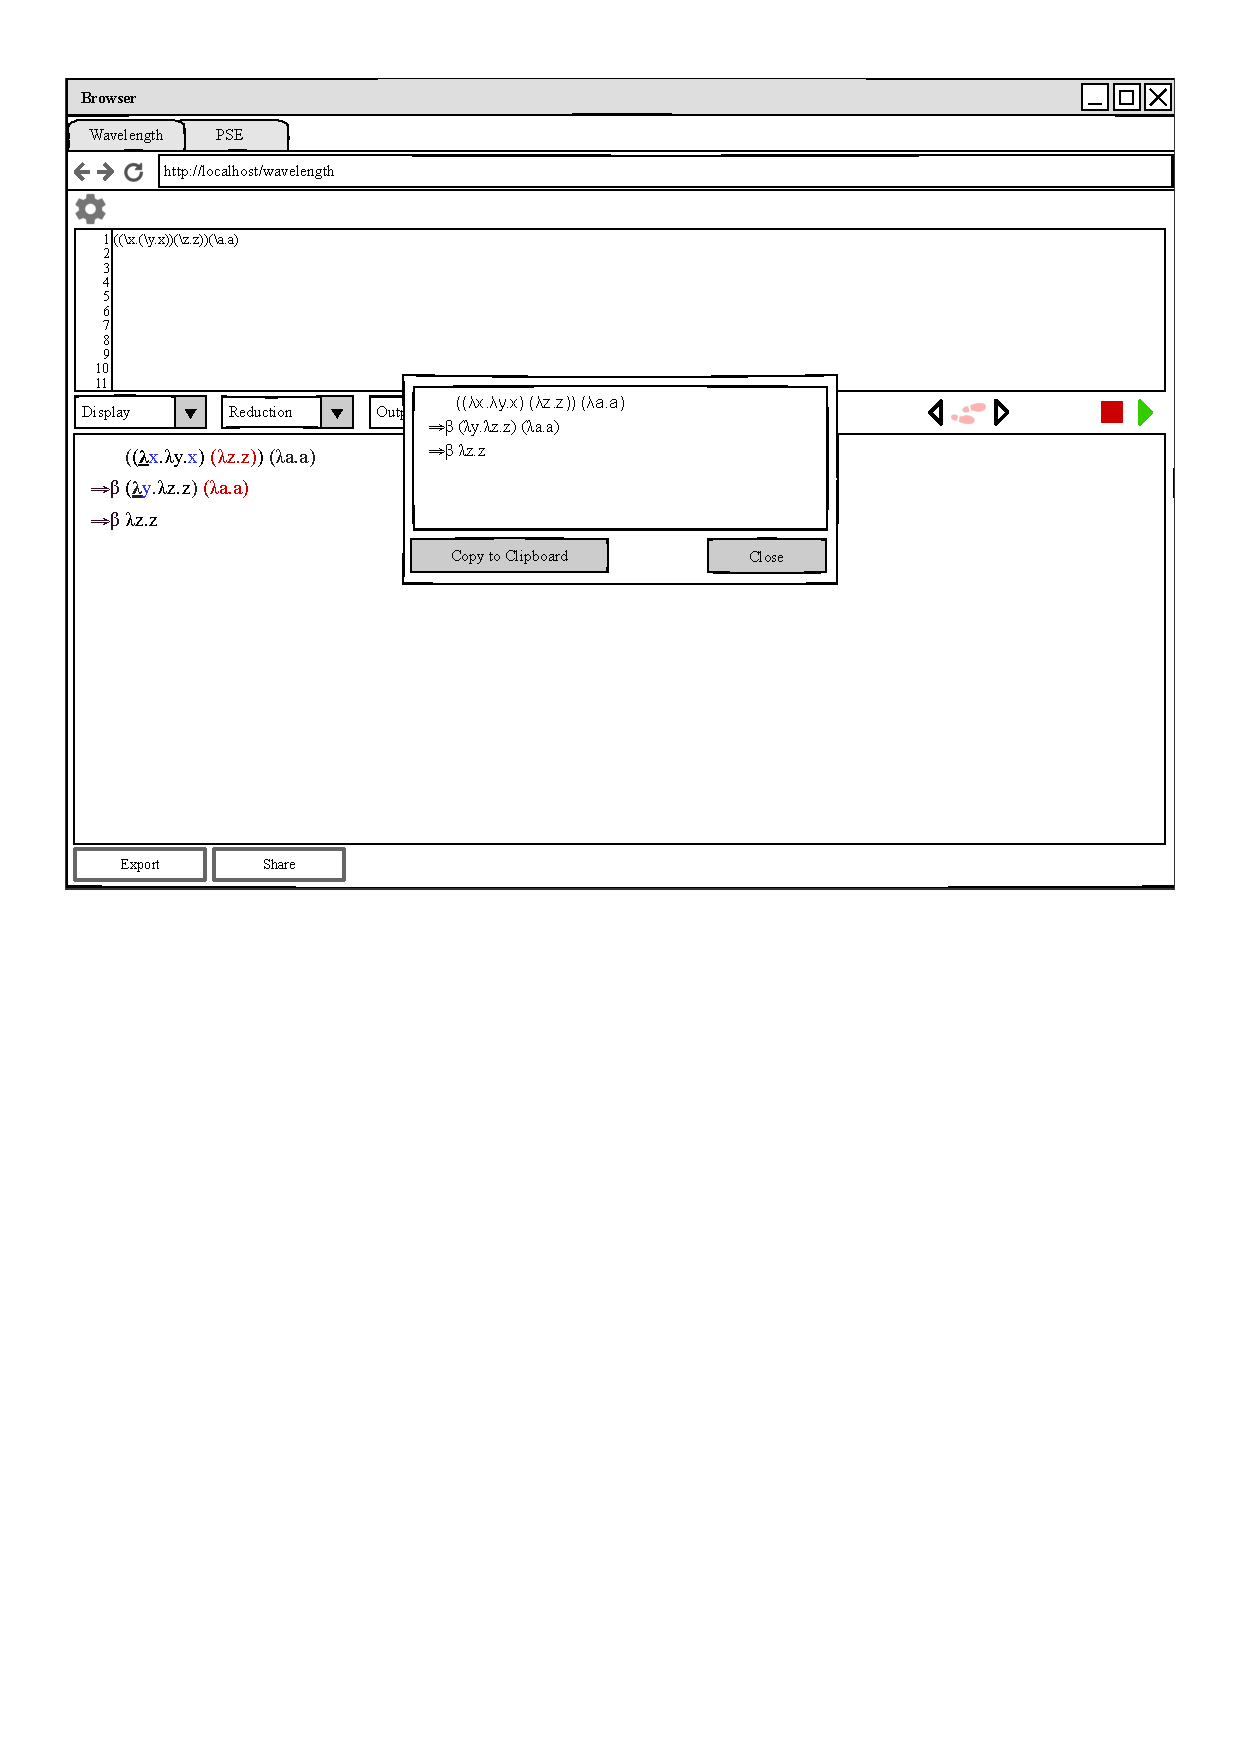
\includegraphics[width=0.75\textwidth]{img/wavelength_export_window_unicode}
	\end{subfigure}
	\caption{\label{fig:export}Durch Klick auf den Export Knopf, kann das aktuelle Ausgabefenster in das gewünschte Format exportiert werden.}
\end{figure}


\begin{figure}[H]
	\centering
	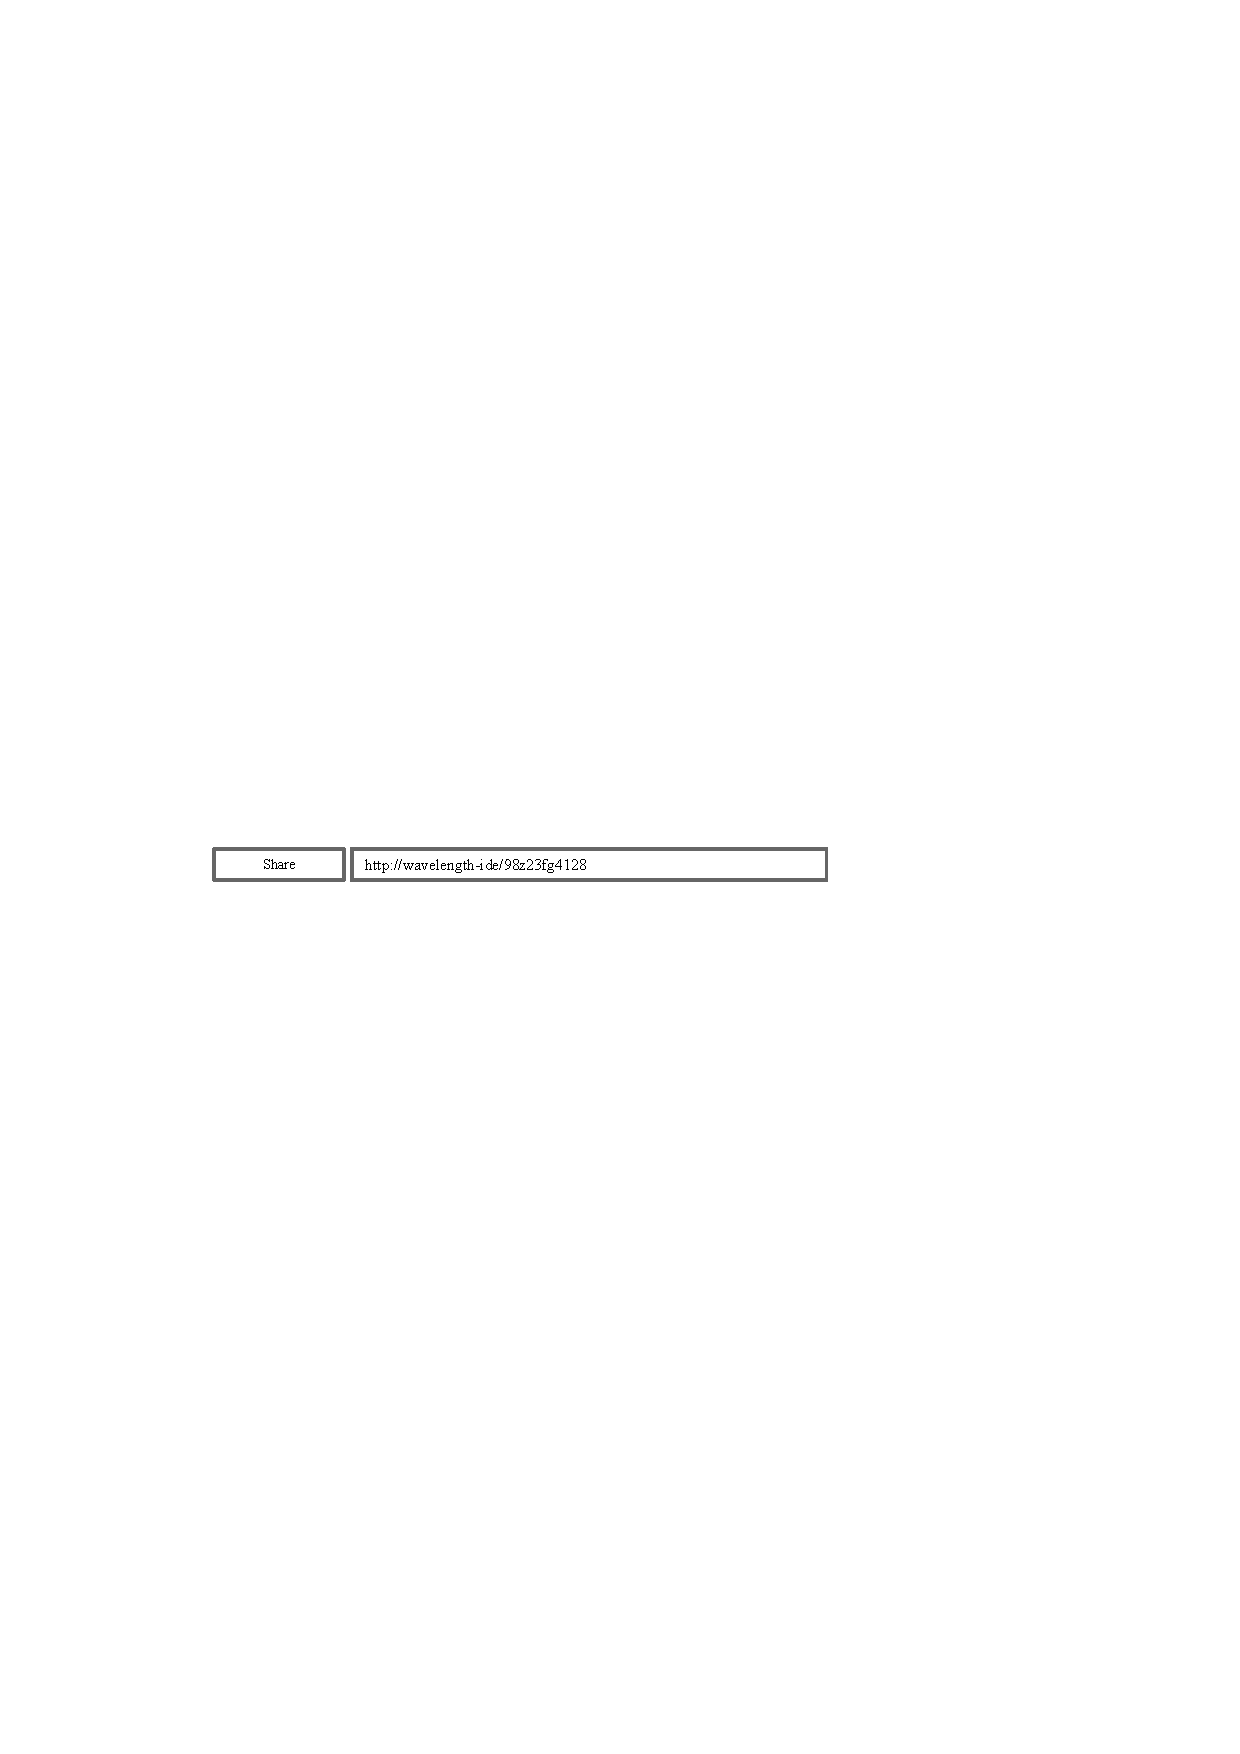
\includegraphics{img/share}
	\caption{Bei Betätigen des Share Knopfes wird ein entsprechender Link erstellt.}
	\label{img:share}
\end{figure}


\begin{figure}[H]
	\centering
	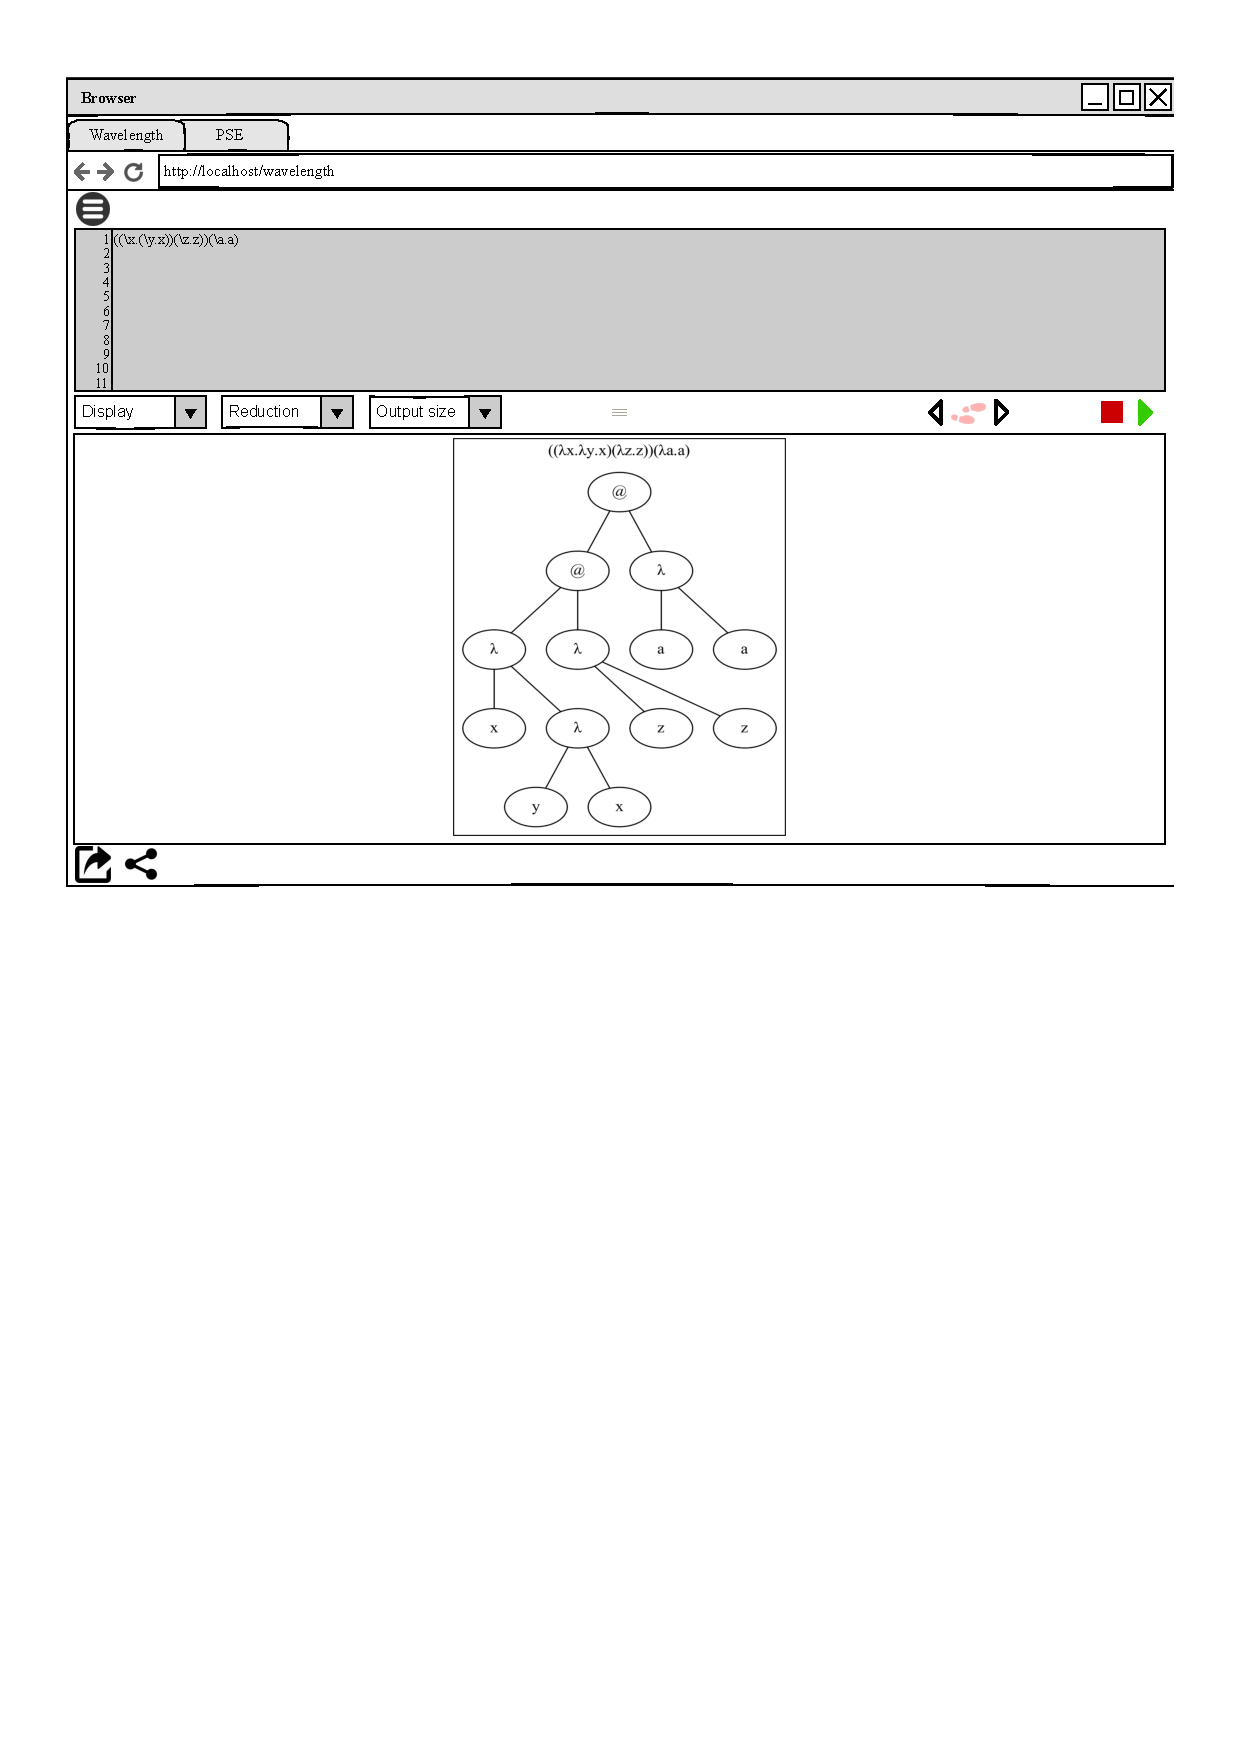
\includegraphics[width=\textwidth]{img/displayTree1}
	\caption{\label{fig:tree}Wird das Darstellungsformat "Tree" ausgewählt (siehe \cref{fig:outputOptions}), so wird der eingegebene \gls{lt} als Syntaxbaum im Ausgabefeld angezeigt.}
\end{figure}


\begin{figure}[H]
	\begin{subfigure}{0.5\textwidth}
		\centering
		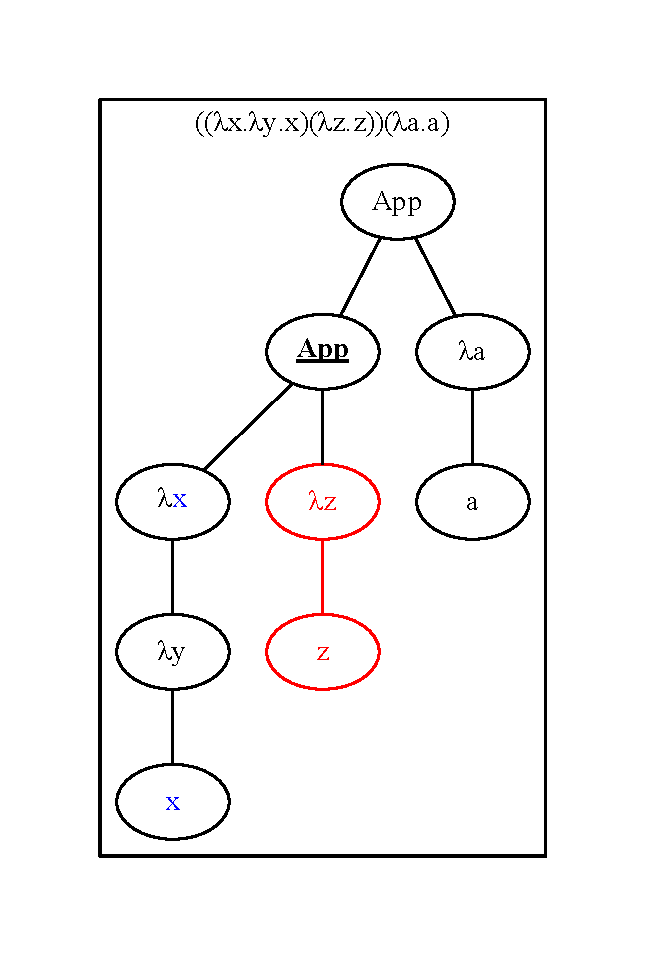
\includegraphics{img/displayTree2}
		\caption{ausgewählte \gls{lapp}}
	\end{subfigure}
	\begin{subfigure}{0.5\textwidth}
		\centering
		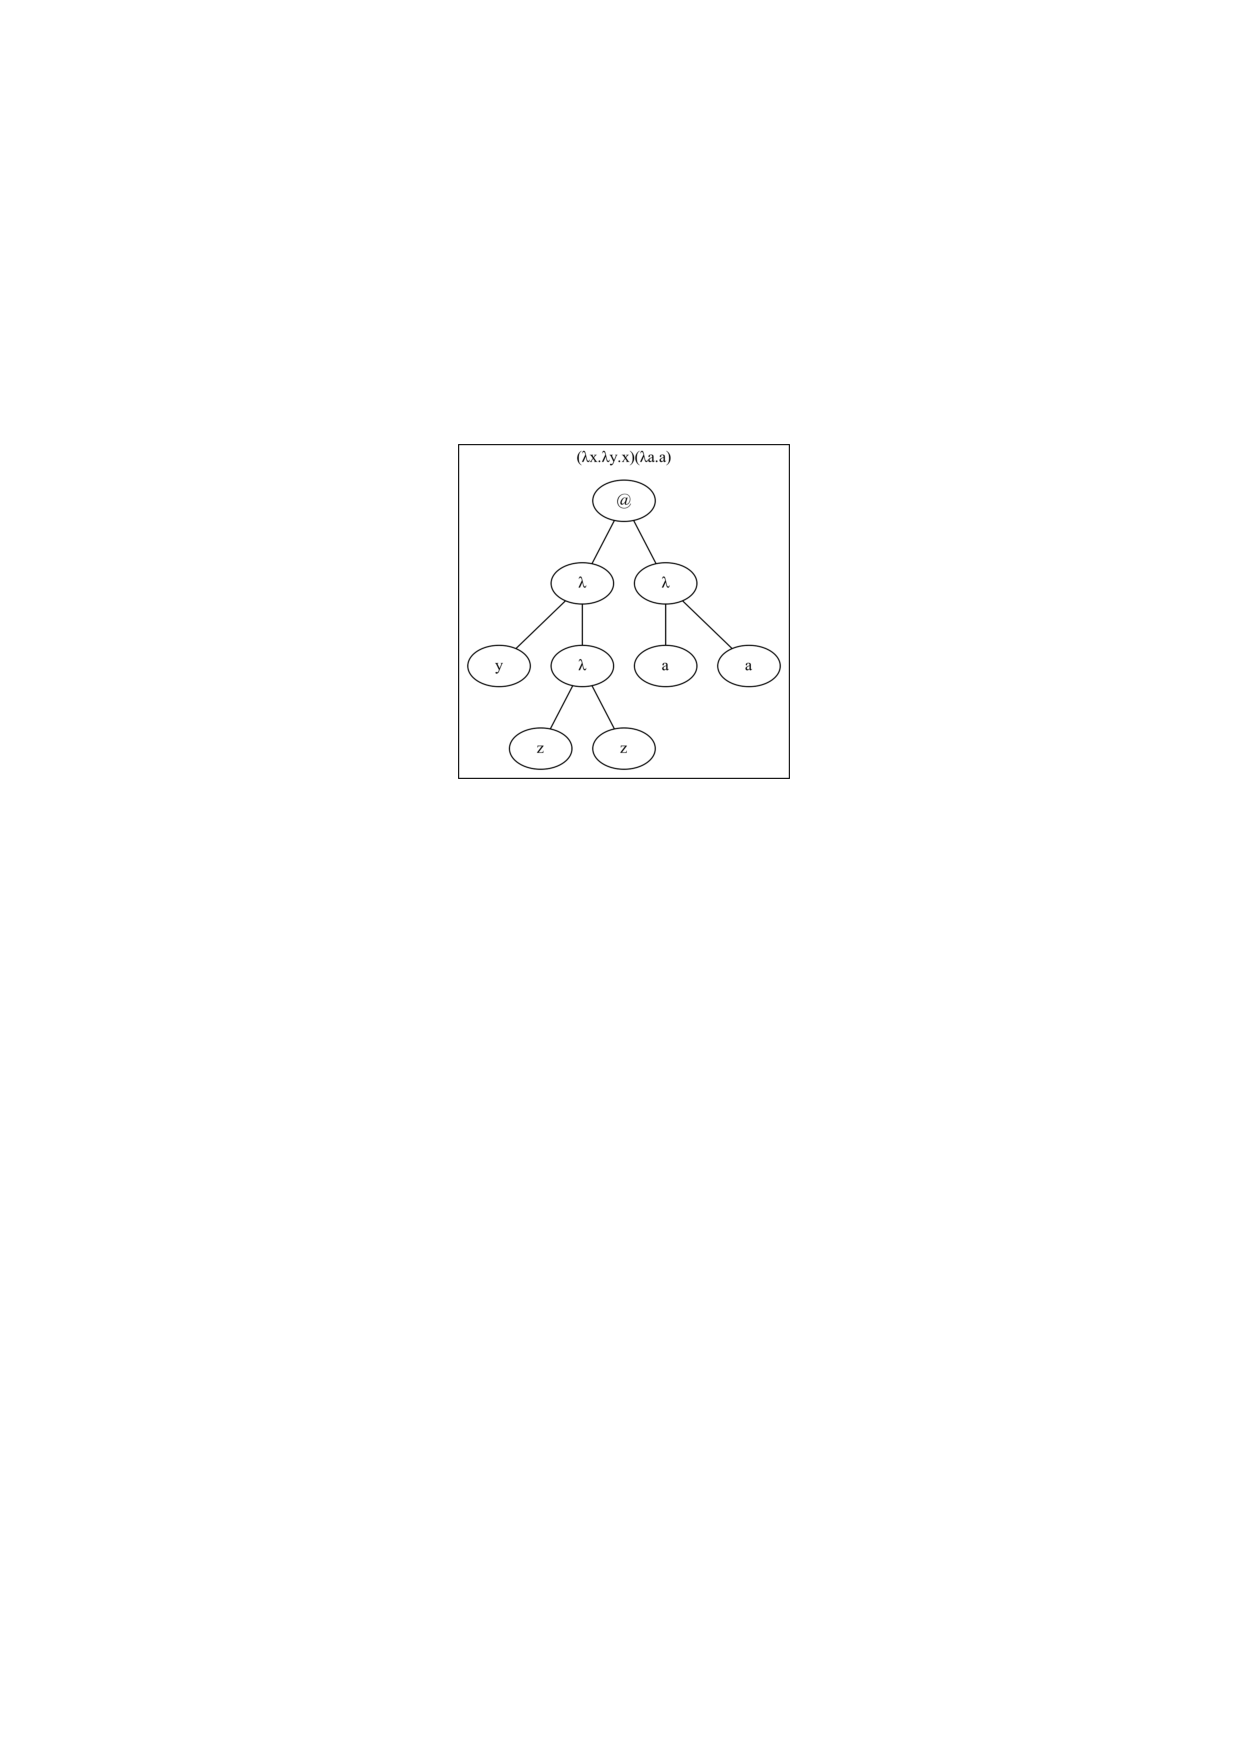
\includegraphics{img/displayTree3}
		\caption{neue Ausgabe}
	\end{subfigure}
	\caption{Wird eine "@"-Symbol (\gls{lapp}) angeklickt, so wird dieser Teilterm als neue Ausgabe angezeigt.}
\end{figure}


\begin{figure}[H]
	\centering
	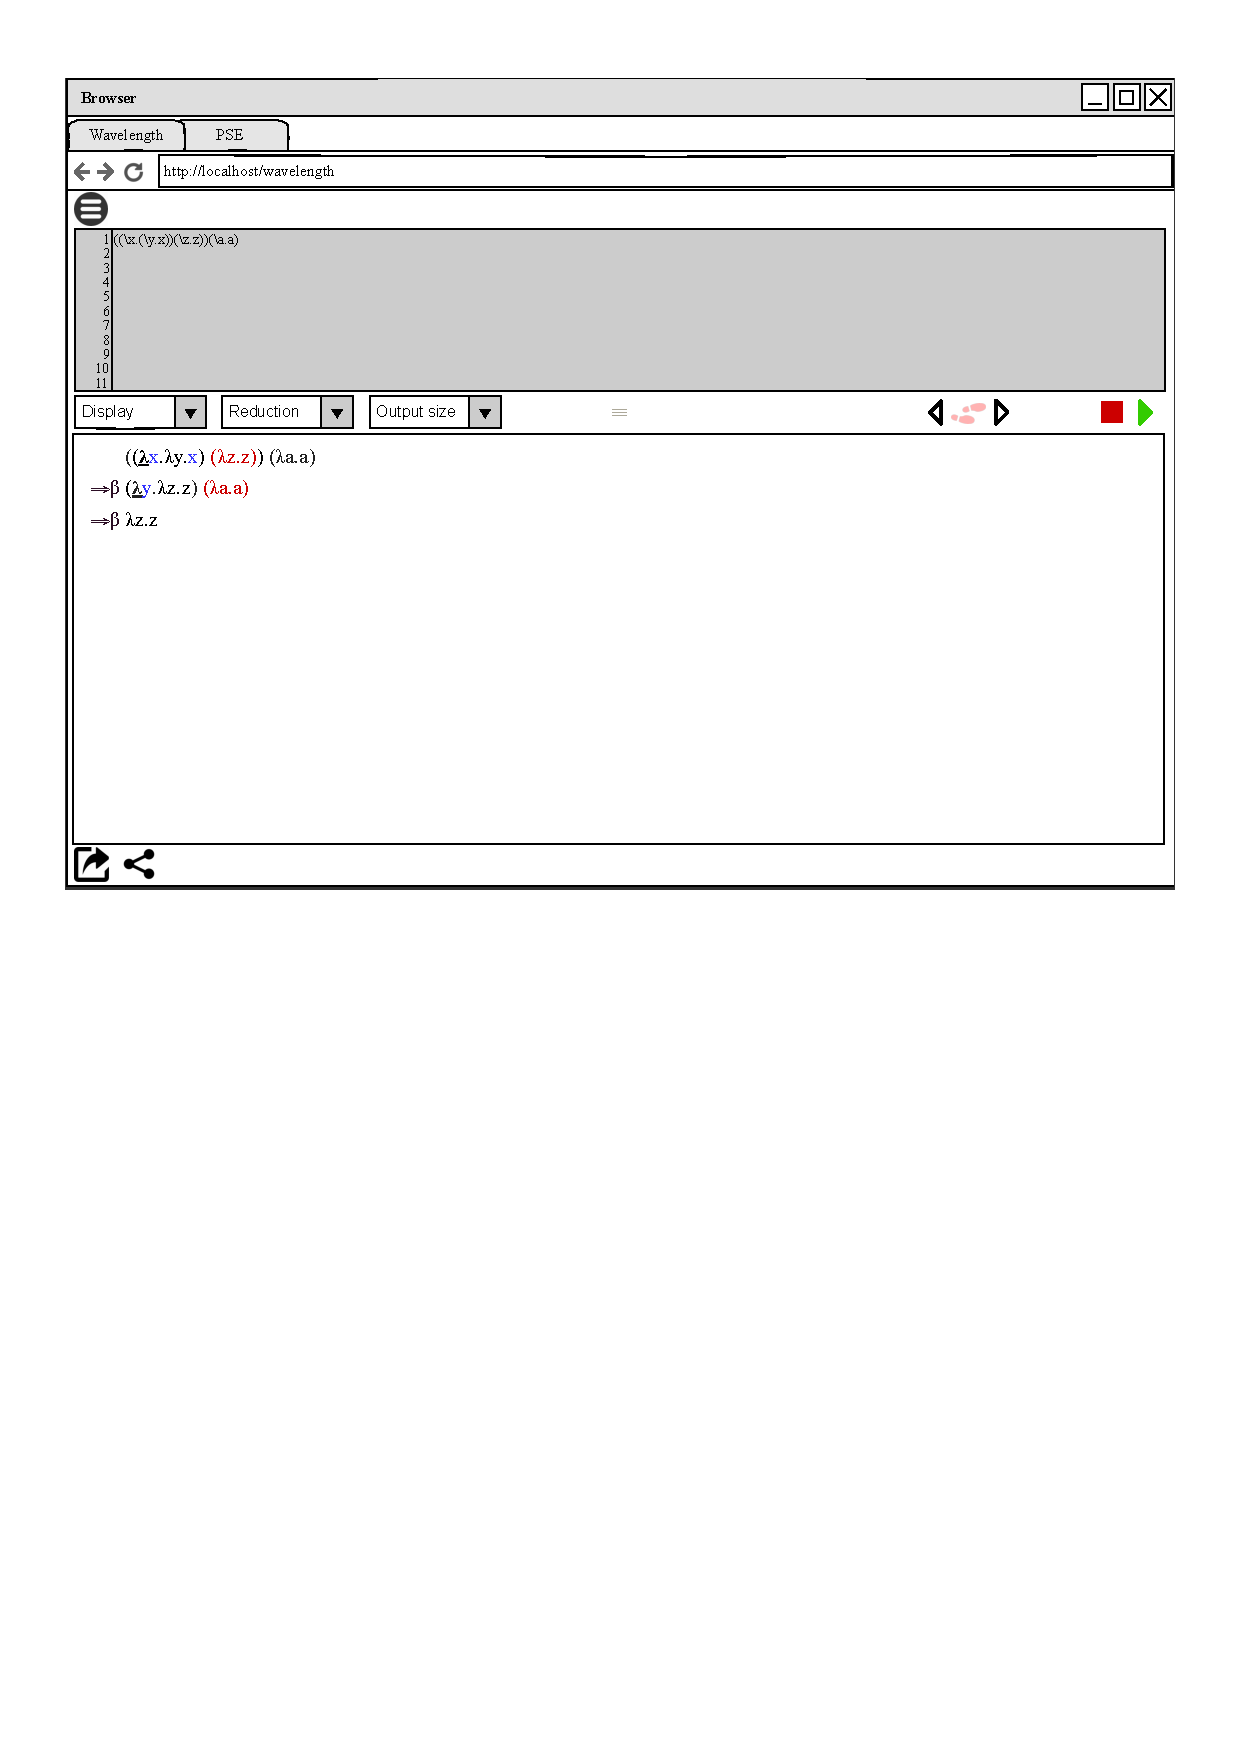
\includegraphics[width=\textwidth]{img/Unicode_Darstellunsgmodus}
	\caption{\label{fig:unicode}Wird das Darstellungsformat "Unicode" ausgewählt (siehe \cref{fig:outputOptions}), so wird der eingegebene \gls{lt} in Unicode im Ausgabefeld angezeigt.}
\end{figure}



%%%%%%%%%
\section{Glossar}

\printglossaries

\end{document}
